% \documentclass[sigconf,review]{acmart}

\documentclass[sigconf,nonacm]{acmart}
\settopmatter{printacmref=false}
\renewcommand\footnotetextcopyrightpermission[1]{}

\settopmatter{authorsperrow=6}


% ---------- Case card environment ----------
\usepackage[most]{tcolorbox}

\newtcolorbox{casecard}[1]{%
  enhanced, breakable,
  colback=white, colframe=black!70,
  boxrule=0.8pt, arc=2mm,
  left=6pt, right=6pt, top=6pt, bottom=6pt,
  title=\textbf{#1}, fonttitle=\bfseries
}


\usepackage{booktabs}
\usepackage{multirow}
\usepackage{amsmath,mathtools}
\usepackage{enumitem}
\usepackage{balance}
\usepackage{placeins}
\usepackage{xcolor}
\usepackage{xspace}
\usepackage{algorithm}
\usepackage[noend]{algpseudocode}
\usepackage{framed}
\usepackage{listings}



\lstset{breaklines=true, basicstyle=\small\ttfamily, breakatwhitespace=false, columns=fullflexible, xleftmargin=0.5em, framexleftmargin=0pt}
\definecolor{shadecolor}{rgb}{0.92,0.92,0.92}
\newenvironment{promptbox}{\begin{shaded}}{\end{shaded}}
\newenvironment{codebox}{\begin{shaded}}{\end{shaded}}

% Prompt boxes (colored, framed) for supplementary material.
\definecolor{promptbg}{RGB}{242,247,255}
\definecolor{promptborder}{RGB}{52,95,175}
\newenvironment{promptcard}[1]{%
  \def\FrameCommand##1{\fcolorbox{promptborder}{promptbg}{##1}}%
  \setlength{\fboxsep}{6pt}%
  \setlength{\fboxrule}{0.6pt}%
  \MakeFramed{\advance\hsize-\width \FrameRestore}%
  \noindent\textbf{#1}\par\medskip\ttfamily\small\raggedright
}{%
  \endMakeFramed
}

% Figures/plots fully in LaTeX (no external images needed)
\usepackage{tikz}
\usetikzlibrary{positioning,arrows.meta,calc,fit,matrix,shapes,shapes.geometric}
\usepackage{pgfplots}
\pgfplotsset{compat=1.18}

% Guard against stale aux files that may contain lineno markers (e.g., \@LN@col).
\makeatletter
\providecommand\@LN@col[1]{}
\makeatother

% ===== Project-level macros (inlined from materials/macros.tex) =====
% ===== Project-level macros =====

% Metrics
\newcommand{\bench}{FinToolBench}
\newcommand{\methodname}{FATR}
\newcommand{\tir}{\textsc{TIR}\xspace}
\newcommand{\tesr}{\textsc{TESR}\xspace}
\newcommand{\cer}{\textsc{CER}\xspace}
\newcommand{\soft}{\textsc{Soft Score}\xspace}
\newcommand{\css}{\textsc{CSS}\xspace}
\newcommand{\tmr}{\textsc{TMR}\xspace}
\newcommand{\imr}{\textsc{IMR}\xspace}
\newcommand{\dmr}{\textsc{DMR}\xspace}

% Convenience
\newcommand{\realt}{\texttt{realtime}}
\newcommand{\dailyt}{\texttt{daily}}
\newcommand{\asfiledt}{\texttt{as\_filed}}
\newcommand{\periodict}{\texttt{periodic}}
\newcommand{\statict}{\texttt{static}}

\newcommand{\informational}{\texttt{informational}}
\newcommand{\advisory}{\texttt{advisory}}
\newcommand{\transactional}{\texttt{transactional}}

\title{FinToolBench: Evaluating LLM Agents for Real-World \\ Financial Tool Use}

% Datasets \& Benchmarks Track is single-blind (non-anonymous): include authors.
\author{Jiaxuan Lu}
\authornote{These authors contributed equally.}
\affiliation{%
  \institution{Shanghai AI Laboratory}
  \country{ }
}

\author{Kong Wang}
\authornotemark[1]
\affiliation{%
  \institution{Hunan University}
  \country{ }
}

\author{Yemin Wang}
\affiliation{%
  \institution{Xiamen University}
  \country{ }
}

\author{Qingmei Tang}
\affiliation{%
  \institution{Tencent}
  \country{ }
}

\author{Hongwei Zeng}
\affiliation{%
  \institution{UCAS}
  \country{ }
}

\author{Xiang Chen}
\affiliation{%
  \institution{Tongji University}
  \country{ }
}

\author{Jiahao Pi}
\affiliation{%
  \institution{Shanghai AI Laboratory}
  \country{ }
}

\author{Shujian Deng}
\affiliation{%
  \institution{Shanghai AI Laboratory}
  \country{ }
}

\author{Lingzhi Chen}
\affiliation{%
  \institution{Shanghai AI Laboratory}
  \country{ }
}

\author{Yi Fu}
\affiliation{%
  \institution{Shanghai AI Laboratory}
  \country{ }
}

\author{Kehua Yang}
\authornote{Corresponding author.}
\affiliation{%
  \institution{Hunan University}
  \country{ }
}

\author{Xiao Sun}
\authornotemark[2]
\affiliation{%
  \institution{Shanghai AI Laboratory}
  \country{ }
}

\renewcommand{\shortauthors}{Lu et al.}

% CCS Concepts and Keywords are mandatory for papers over two pages in acmart.
\begin{CCSXML}
<ccs2012>
 <concept>
  <concept_id>10002951.10003260.10003261</concept_id>
  <concept_desc>Information systems~Information retrieval</concept_desc>
  <concept_significance>300</concept_significance>
 </concept>
 <concept>
  <concept_id>10010147.10010257</concept_id>
  <concept_desc>Computing methodologies~Machine learning</concept_desc>
  <concept_significance>300</concept_significance>
 </concept>
 <concept>
  <concept_id>10002951.10003317.10003331</concept_id>
  <concept_desc>Information systems~Data mining</concept_desc>
  <concept_significance>300</concept_significance>
 </concept>
</ccs2012>
\end{CCSXML}
\ccsdesc[300]{Information systems~Information retrieval}
\ccsdesc[300]{Computing methodologies~Artificial intelligence}
\ccsdesc[300]{Applied computing~Economics}
\keywords{LLM Agents, Tool Use, Financial Benchmarks, Real-World APIs}

\begin{abstract}
The integration of Large Language Models (LLMs) into the financial domain is driving a paradigm shift from passive information retrieval to dynamic, agentic interaction. While general-purpose tool learning has witnessed a surge in benchmarks, the financial sector, characterized by high stakes, strict compliance, and rapid data volatility, remains critically underserved. Existing financial evaluations predominantly focus on static textual analysis or document-based QA, ignoring the complex reality of tool execution. Conversely, general tool benchmarks lack the domain-specific rigor required for finance, often relying on toy environments or a negligible number of financial APIs. To bridge this gap, we introduce \textbf{\bench}, the first real-world, runnable benchmark dedicated to evaluating financial tool learning agents. Unlike prior works limited to a handful of mock tools, \bench{} establishes a realistic ecosystem coupling 760 executable financial tools with 295 rigorous, tool-required queries. We propose a novel evaluation framework that goes beyond binary execution success, assessing agents on finance-critical dimensions: timeliness, intent type, and regulatory domain alignment. Furthermore, we present \textbf{FATR}, a finance-aware tool retrieval and reasoning baseline that enhances stability and compliance. By providing the first testbed for auditable, agentic financial execution, \bench{} sets a new standard for trustworthy AI in finance. The tool manifest, execution environment, and evaluation code will be open-sourced to facilitate future research.
\end{abstract}

\begin{document}
\maketitle



\begin{figure}[t]
\centering
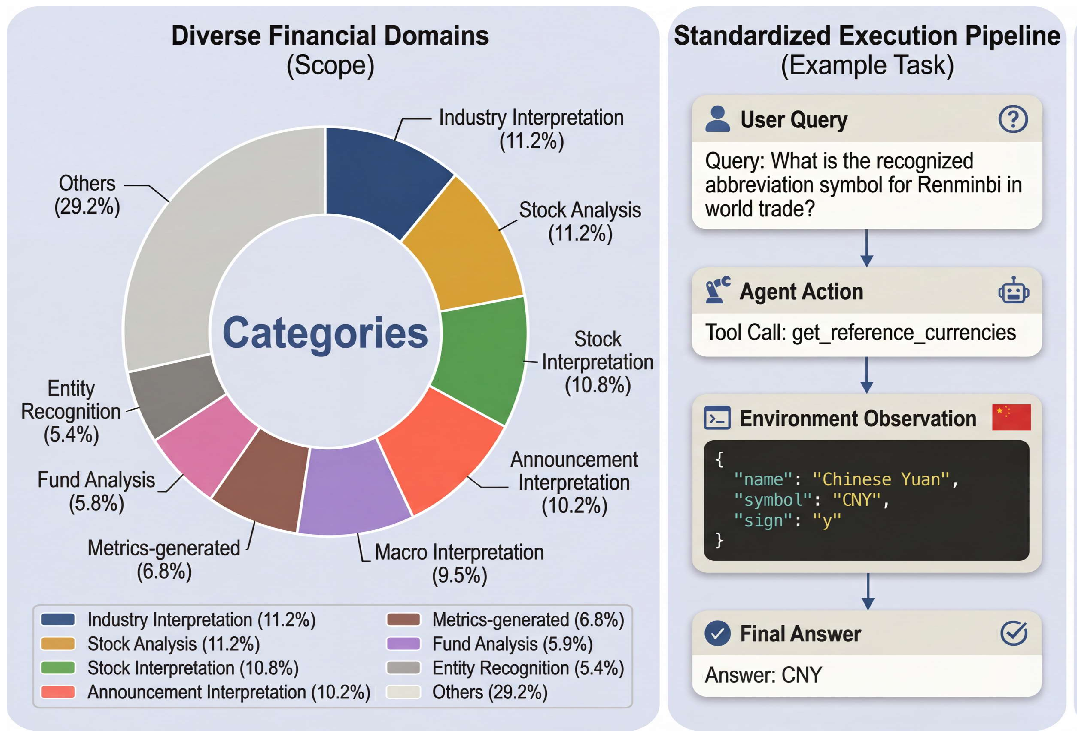
\includegraphics[width=\columnwidth]{first_page.pdf}
\caption{FinToolBench overview. Left: the scope of our benchmark  across representative categories. Right: an example of the standardized execution pipeline, where an LLM agent selects a tool, observes the environment output, and produces a final answer with an auditable tool trace.}
\Description{FinToolBench overview figure showing a breakdown of 760 tools by category and an example tool-execution pipeline from user query to tool call, environment observation, and final answer.}
\label{fig:overview}
\end{figure}

\section{Introduction}
The integration of Large Language Models (LLMs) is driving a revolution in the financial industry, moving beyond static analysis to dynamic, autonomous interaction.
Tool-using LLM agents are increasingly deployed as interfaces to financial data, translating natural-language requests into a sequence of API calls, database queries, and computations.
This evolution promises to democratize access to sophisticated market analysis, yet it introduces risks that are unique to the domain.
In this setting, a wrong tool call can be more damaging than a wrong free-form answer because it can look grounded while relying on stale data, drifting endpoints, or a mismatched market domain~\cite{guo2024stabletoolbench}.
Evaluation must therefore assess not only whether tools are invoked and executed successfully, but also whether the resulting tool trace is acceptable under finance-specific constraints that practitioners actually care about.
More broadly, recent work is moving toward agents that operate over longer horizons and in settings where tool use itself can evolve, which further increases the value of trace-level evaluation~\cite{lu2026beyondstatictools,jiang2025scp}.

Despite rapid progress on tool-augmented reasoning, existing benchmarks leave a gap between what is easy to measure and what is necessary to trust.
General tool benchmarks emphasize API correctness and executability, and they have begun to confront instability in real environments~\cite{guo2024stabletoolbench}, but they rarely test finance-specific acceptability constraints.
Existing finance benchmarks, in contrast, typically focus on knowledge- or document-centric QA. However, they suffer from a critical deficiency: they involve virtually no executable tools, relying instead on static datasets or a negligible number of mock interfaces.
As a result, it remains hard to distinguish an agent that executes correctly from one whose tool choices are acceptable under timeliness, intent restraint, and domain alignment.
We argue that current metrics are blind to three recurring failure modes essential for financial reliability.
First, \textit{timeliness} is often implicit in finance, \textit{e.g.}, a question asking for ``current'' exchange rates is fundamentally unanswered if the agent retrieves a daily snapshot, even if the API call is syntactically perfect.
Second, \textit{intent restraint} is critical, \textit{i.e.}, an agent must strictly differentiate between informational queries and transactional actions, ensuring it never escalates to execution without explicit authorization.
Third, \textit{domain alignment} is essential, \textit{i.e.}, the chosen tool chain must strictly adhere to the regulatory and market domain of the query (\textit{e.g.}, utilizing equity market tools for a cryptocurrency inquiry is a hallucination of domain).

To address these gaps, we introduce \textbf{\bench}, a runnable benchmark built from real free-tier tools and tool-required questions.
\bench{} represents a significant scaling of financial agent evaluation, comprising a tool library of 760 executable tools and a question set of 295 items, \textit{i.e.}, 166 single-tool and 129 multi-tool.
Crucially, each tool is annotated with three finance attributes, \textit{i.e.}, timeliness, intent type, and regulatory domain, enabling us to compute call-level compliance mismatch rates, \textit{i.e.}, \tmr{}, \imr{}, \dmr{}, alongside standard invocation and execution metrics.
To demonstrate the utility of this benchmark, we also propose \textbf{FATR} (Finance-Aware Tool Retrieval), a lightweight baseline.
FATR addresses the specific challenges of the financial domain by retrieving a small candidate set, injecting finance attributes into tool cards, and stabilizing execution with caching, retries, and output compression.
Figure \ref{fig:overview} provides a snapshot of the benchmark scope and the standardized execution pipeline we evaluate, from user query to tool call, environment observation, and a trace-backed final answer.

Our contributions are summarized as follows:
\begin{enumerate}[leftmargin=*]
\item \textbf{FinToolBench:} A benchmark of 760 free-tier financial tools and 295 tool-required questions that produces auditable tool traces and evaluates tool use under real execution conditions.
\item \textbf{Finance-Aware Evaluation:} We propose a novel set of capability metrics plus call-level compliance mismatch rates (\tmr{}, \imr{}, \dmr{}) that specifically measure violations of timeliness, intent restraint, and domain alignment.
\item \textbf{FATR Baseline:} We introduce a lightweight baseline that injects finance attributes into tool cards and improves stability, providing a strong reference point for future work on trustworthy financial agents.
\end{enumerate}


\section{Related Work}\label{sec:related}
\subsection{Tool-Using Agents and Benchmarks}
Tool-augmented agents interleave reasoning with external actions to improve grounding and support up-to-date answers.
ReAct \cite{yao2022react} and Toolformer \cite{schick2023toolformer} are representative examples, and recent systems connect LLMs to large tool inventories and external APIs \cite{patil2024gorilla,qin2023toolllm}.
Correspondingly, benchmarks evaluate whether models can select and call tools at scale, including API-Bank \cite{li2023api} and StableToolBench \cite{guo2024stabletoolbench}.
Beyond API-centric suites, agent benchmarks emphasize long-horizon interaction in realistic environments, including AgentBench \cite{liu2023agentbench}, GAIA \cite{mialon2023gaia}, WebArena \cite{zhou2023webarena}, WorkArena \cite{drouin2024workarena}, and $\tau$-bench \cite{narasimhan2024tau}.
Recent efforts further sharpen the evaluation focus toward tool-interface competence and agentic behavior. BFCL studies function-calling and tool-use evaluation under controlled protocols~\cite{patilberkeley}, and $\tau^2$-bench extends the setting to dual-control conversational environments that stress interaction and coordination~\cite{barres2025tau2}.
Concurrent work studies agents in settings where tools or capabilities evolve over time and where long-horizon traces are central artifacts. Beyond Static Tools investigates test-time tool evolution for scientific reasoning~\cite{lu2026beyondstatictools}, and SCP explores a global web of autonomous scientific agents for discovery~\cite{jiang2025scp}. DeepResearch Arena provides an evaluation setting for research-oriented agents grounded in seminar tasks~\cite{wan2025deepresearcharena}, and multi-agent evidence-based reasoning further motivates trace-centric diagnostics~\cite{yang2025fromwhat}.

\subsection{Financial Benchmarks and Evaluation}
In finance, most benchmarks emphasize domain knowledge and document-centric QA rather than executable tool use. Examples include FinanceBench~\cite{islam2023financebench}, OpenFinData~\cite{openfindata2023github}, and report-focused datasets such as FinQA~\cite{chen2021finqa} and TAT-QA~\cite{zhu2021tat}. While recent works like FinEval~\cite{guo2025fineval}, FLAME~\cite{guo2025flame}, and the Finance Agent Benchmark~\cite{bigeard2025finance} broaden knowledge coverage, critical limitations remain. For instance, although the Finance Agent Benchmark incorporates tool use for accessing filings, it neither releases a standardized large tool library nor defines call-level compliance metrics. Consequently, most datasets represent a "static" paradigm that stops at the final answer, failing to evaluate the executability and acceptability of tool traces under essential finance constraints, such as timeliness, intent restraint, and market-domain alignment. \bench{} addresses this by providing an execution-grounded environment that pairs a fully runnable tool inventory with tool-required questions, moving beyond static QA to support agentic workflows that require real-time data retrieval and multi-step reconciliation.

Recent safety-oriented agent evaluations highlight complementary concerns about the risks of tool use, including prospective safety benchmarks and web-agent benchmarks that probe deliberate misuse~\cite{xia2025safetoolbench,tur2025safearena}. However, these evaluations are not finance-specific and do not operationalize domain-grounded constraints like timeliness, intent limits, and regulatory scope. \bench{} targets this gap by explicitly defining finance constraints at the level of each tool call using a lightweight, auditable attribute schema. To our knowledge, this makes \bench{} the first finance benchmark to enable direct measurement of timeliness, intent, and domain mismatches from execution traces, rather than relying solely on final answer correctness or generic safety checks.

\begin{figure*}[t]
\centering
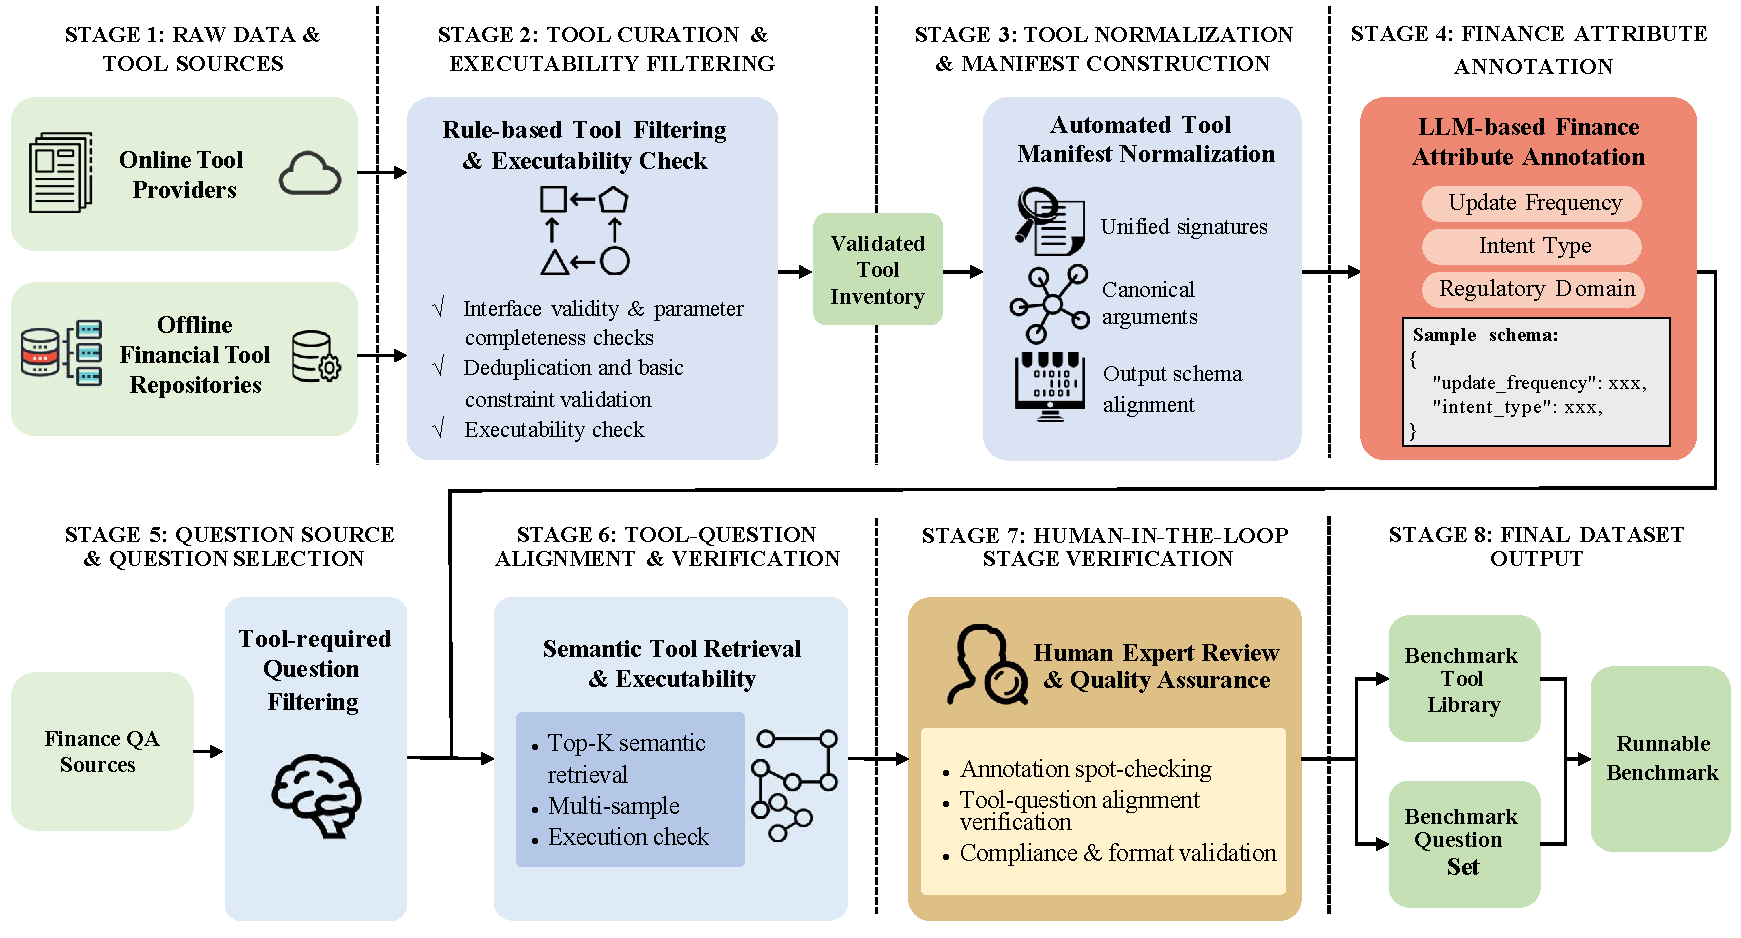
\includegraphics[width=\textwidth]{dataset_construction.pdf}
\caption{FinToolBench dataset construction pipeline. Stage 1 collects raw tool sources. Stage 2 performs tool curation and executability filtering to obtain a validated tool inventory. Stage 3 normalizes tools into a unified manifest with standardized signatures, canonical arguments, and aligned output schemas. Stage 4 annotates each tool with finance attributes (timeliness, intent type, regulatory domain). Stage 5 sources and selects tool-required questions. Stage 6 aligns questions with tools via semantic retrieval, multi-sample verification, and execution checks. Stage 7 adds human-in-the-loop quality assurance. Stage 8 outputs the benchmark tool library and benchmark question set as a runnable benchmark.}
\Description{Overview of the eight-stage FinToolBench construction pipeline from tool sources and curation through manifest normalization, finance attribute annotation, question selection, tool-question alignment, human verification, and final benchmark outputs.}
\label{fig:data_pipeline}
\end{figure*}

\subsection{Evaluation Standard}
Because answer correctness is hard to score at scale for open-ended questions, recent work uses LLMs as judges with structured rubrics, including MT-Bench~\cite{zheng2023judging} and G-Eval~\cite{liu2023g}. FinToolBench adopts repeated judging and reports both capability and compliance so that execution failures can be separated from evaluation uncertainty~\cite{zheng2023judging,liu2023g}.
At the same time, recent studies show that LLM-based scoring can be unstable across runs and sensitive to prompting and evaluation design, which motivates calibration and robustness checks when using judges as measurement instruments~\cite{hashemi2024llmrubric,haldar2025ratingroulette}.
Domain-specific judge frameworks also emphasize evidence-anchored rubrics.
They also test evaluator robustness under distribution shift~\cite{dsouza2025yescieval}.
In line with these findings, we reduce variance via repeated judging and explicitly separate tool execution from correctness, so that a failure to call or execute tools is not conflated with an evaluation artifact.
Finally, recent work suggests that comparative setups can elicit more informative judgments than independent scoring by exposing missing evidence through contrastive context~\cite{zhang2025crowdcomparative}.
Our protocol is compatible with such improvements, since the benchmark produces complete tool traces that can be inspected and re-judged under alternative rubric designs.




\section{FinToolBench}
\label{sec:benchmark}

FinToolBench is an execution-grounded benchmark designed to evaluate financial tool use under real execution.
Its design emphasizes two principles.
First, every run produces an auditable tool trace.
Second, evaluation separates capability (\textit{i.e.}, invocation and execution success) from compliance (\textit{i.e.},  call-level timeliness, intent, and domain alignment).
The benchmark measures an agent's ability to select tools from a large heterogeneous library, instantiate valid arguments, handle execution failures, and produce answers whose tool use respects finance-specific constraints.

In contrast to prior tool-use benchmarks that focus primarily on API calling accuracy, FinToolBench evaluates both capability and compliance directly from executable tool traces.
Figure~\ref{fig:data_pipeline} summarizes the construction pipeline.
Concretely, we follow the staged process in Figure~\ref{fig:data_pipeline} to produce both a validated tool inventory and a tool-required question set.
The pipeline has eight stages.
Stages 1--4 cover Raw Data \& Tool Sources, Tool Curation \& Executability Filtering, Tool Normalization \& Manifest Construction, and LLM-based Finance Attribute Annotation.
Stages 5--8 cover Question Source \& Question Selection, Tool-Question Alignment \& Verification, Human-in-the-Loop Stage Verification, and Final Dataset Output.
The design for evaluation follows lines of work that stress end-to-end tool selection, argument construction, and trace-based diagnosis under real execution.

% ======================================================
\subsection{Tool Inventory}
\label{subsec:tool_inventory}

\subsubsection{Tool Sources}
\label{subsec:tool_sources}

We construct the tool inventory from two complementary tool ecosystems with different reliability and documentation characteristics.
We restrict to free-tier sources so that the benchmark is reproducible without proprietary data contracts. 

\paragraph{RapidAPI}
RapidAPI hosts a large marketplace of third-party APIs, providing broad coverage of real-time and web-based services. Free-tier access typically requires API keys.

\paragraph{AkShare.}
AkShare is an open-source Python library for programmatic access to financial data. It offers stable, research-oriented interfaces covering a wide range of financial domains.
Together, these two sources provide complementary coverage: RapidAPI emphasizes diversity and real-time accessibility, while AkShare offers reliable and well-documented financial data interfaces.
% ------------------------------------------------------
\subsubsection{Tool Curation and Executability Filtering}
\label{subsec:executability}

\paragraph{RapidAPI}
We filter raw RapidAPI endpoints using a rule-based executability pipeline.
A tool is retained only if it satisfies all of the following criteria:

\begin{itemize}
  \item \textbf{Interface validity:} complete parameter definitions and non-empty descriptions.
  \item \textbf{Deduplication:} removal of duplicate names and semantically identical interfaces.
  \item \textbf{Rate-limit sufficiency:} enforcement of minimum rate limits (e.g., 10/hour, 100/day, 300/month).
  \item \textbf{Authentication feasibility:} executable under free-tier access.
  \item \textbf{Runtime executability:} at least one successful test invocation.
\end{itemize}

Endpoints with broken URLs, insufficient rate limits, undocumented or faulty authentication flows,
or persistent execution failures are discarded, which ensures that all RapidAPI tools included in FinToolBench are executable and reliable during evaluation.

\paragraph{AkShare.}
We select AkShare interfaces using finance-related function-name cues
(\textit{e.g.}, stock, fund, bond, futures, option, index, macro, currency, crypto, rate, treasury, ETF),
and verify executability through direct invocation.


\paragraph{Scale.}
We start from 5{,}470 candidate interfaces (4{,}507 RapidAPI endpoints and 963 AkShare interfaces).
After filtering RapidAPI endpoints and selecting AkShare interfaces,
the final tool library contains 760 tools.
The full criteria and counts are given in appendix~\ref{sec:tool_curation}.

% ------------------------------------------------------
\subsubsection{Tool Normalization and Manifest Construction}
\label{subsec:normalization}

To make the heterogeneous tool ecosystem amenable to retrieval,
planning, and evaluation, we normalize each tool
into a unified manifest schema.
Each tool manifest includes:
(i) a stable identifier,
(ii) a short description,
(iii) a machine-readable signature with canonicalized parameter names and types.
Normalization reduces avoidable agent errors: date and time fields follow consistent formats,
common identifiers (\textit{e.g.}, tickers) document explicit market conventions,
and output schemas are aligned across sources.

\paragraph{Tool traces.}
During the evaluation process, \bench{} enforces rigorous logging to ensure transparency and reproducibility. Every tool invocation initiated by the agent is captured as a structured execution trace, which constitutes the atomic unit of auditing, error diagnosis, and compliance evaluation. As detailed in Table~\ref{tab:trace_schema}, each record preserves the chronological context through a sequential \texttt{step} index, allowing for the reconstruction of the agent's reasoning chain in multi-turn workflows. The schema also captures the specific \texttt{tool\_name} and the exact JSON-formatted \texttt{parameters} generated by the model, which are critical for detecting hallucinated or malformed inputs. Furthermore, both the raw \texttt{output} and execution \texttt{error} states are logged to differentiate between model reasoning errors and system-level failures such as API rejections.


\begin{table*}[t]
\centering
\caption{Finance attribute schema used in FinToolBench.}
\label{tab:attrs}
\small
\begin{tabular*}{\textwidth}{@{}@{\extracolsep{\fill}}p{0.24\textwidth}p{0.30\textwidth}p{0.38\textwidth}@{}}
\toprule
Attribute & Values & Evaluation role \\
\midrule
\texttt{update\_frequency} &
\realt, \dailyt, \asfiledt, \periodict, \statict &
Penalize stale calls when timeliness is required. \\
\texttt{intent\_type} &
\informational, \advisory, \transactional &
Penalize escalation beyond user intent. \\
\texttt{regulatory\_domain} &
set-valued &
Penalize domain-mismatched tool usage. \\
\bottomrule
\end{tabular*}
\end{table*}

\begin{table}[t]
\centering
\caption{Normalized tool-trace fields.}
\label{tab:trace_schema}
\small
\begin{tabular*}{\columnwidth}{@{}@{\extracolsep{\fill}}p{0.25\columnwidth}p{0.65\columnwidth}@{}}
\toprule
Field & Description \\
\midrule
\texttt{step} & The sequential order of the call within the multi-turn process. \\
\texttt{tool\_name} & The identifier of the specific tool invoked (\textit{e.g.}, \texttt{symbols\_sec\_filings}). \\
\texttt{parameters} & The JSON-formatted arguments generated by the model. \\
\texttt{output} & The tool response, including data or structured error messages. \\
\texttt{error} & Overall execution status, which captures null or specific system-level failures. \\
\bottomrule
\end{tabular*}
\end{table}

% ------------------------------------------------------
\subsubsection{Finance Attribute Annotation}
\label{subsec:finance_attributes}
Financial constraints are frequently implicit within user queries, rendering compliance measurement impossible based on raw execution traces alone. To bridge this gap, \bench{} incorporates a lightweight finance attribute schema that explicitly annotates every tool in the library. The structured metadata enables both the baseline methods outlined in Section~\ref{sec:method} and the quantitative evaluation metrics in Eq.~\eqref{eq:mismatch} to rigorously assess operational acceptability.

As summarized in Table~\ref{tab:attrs}, each tool is categorized along three distinct dimensions. These annotations are generated through an LLM-based labeling pipeline utilizing a three-vote majority agreement protocol to ensure consistency. Comprehensive details regarding the labeling rubric and extended attributes, such as data sensitivity and compliance risk, are provided in Appendix~\ref{sec:attributes}. By embedding these constraints directly into the tool definitions, our design decouples compliance standards from the agent under test, facilitating precise, trace-level auditing of domain mismatches.


% ======================================================
\subsection{Question Set Construction}
\label{subsec:questions}

\subsubsection{Question Source and Question Selection}
\label{subsec:question_sources}

Tool-required questions are adapted from existing finance QA datasets, including the FinanceBench \cite{islam2023financebench} and the OpenFinData (dataset identifier \texttt{openfindata\_}\allowbreak\texttt{release}) \cite{openfindata2023github}.
We standardize all sources into a unified \texttt{\{question, answer, category\}} format by concatenating the original category fields with the question text when needed.
We retain only questions that are identified by Qwen3-8B as requiring tool calls, with the question length limited to 500 characters.
The construction pipeline, including retrieval, verification, and deduplication, is detailed in the appendix (Appendix~\ref{sec:questions}).

\subsubsection{Tool-required Question Filtering}
\label{subsec:tool_required}

To ensure that \bench{} strictly evaluates the model's ability to utilize external tools rather than its reliance on internal parametric memory, we implement a rigorous filtering protocol for candidate questions.
Queries that can be accurately answered via static knowledge or common memorization are systematically excluded, which is critical in the financial domain, where data is often dynamic or proprietary.
Consequently, we retain only those questions that necessitate the retrieval of real-time market data, specific regulatory filings, or quantitative calculations.

\subsubsection{Tool-Question Alignment and Verification}
\label{subsec:alignment}

We employ a robust two-stage pipeline to establish and verify the ground-truth alignment between questions and tools.
First, for each candidate question, we perform a coarse-grained retrieval of the top-20 relevant tools using BGE-M3 dense embeddings~\cite{chen2024bge}.
Second, to refine this set, we apply an LLM-based verification step using Qwen3-8B. We utilize a three-sample majority voting mechanism, retaining only those tools that receive at least two votes to ensure high-confidence alignment.
To mitigate distribution skew and prevent the benchmark from being dominated by a few high-frequency tools, we group single-tool questions by tool name and cap them at two randomly selected questions per tool.
Conversely, multi-tool questions, which represent more complex reasoning chains, are fully retained without deduplication to preserve the diversity of agentic workflows.

\subsubsection{Human-in-the-Loop Verification}
\label{subsec:human_verification}

While the scale of the benchmark necessitates a reliance on automated retrieval and majority-vote labeling, we integrate a human-in-the-loop validation phase to ensure data quality.
We conduct a rigorous spot-check evaluation where domain experts manually verify a statistically significant sample of the dataset.
The audit focuses on two key aspects: confirming the logical necessity of the aligned tools for the given queries and validating the consistency of the attribute annotations.
Furthermore, we check for compliance with execution assumptions and output formatting.
This hybrid approach balances the scalability of automated generation with the reliability of expert oversight, providing a high degree of confidence in the benchmark's validity.


% ======================================================
\subsection{Final Benchmark and Evaluation Protocol}
\label{subsec:final_benchmark}

The final benchmark comprises a unified tool library and a question set.
The tool library contains 760 tools, and the question set contains 295 questions, including 166 single-tool and 129 multi-tool.
Each evaluation run produces a final answer and a complete tool trace, enabling joint assessment of capability, and finance compliance.

\subsection{Evaluation Metrics}
\label{subsec:bench_metrics}

We evaluate each run using two groups of metrics derived from the same auditable tool trace: capability, and compliance.
Capability measures whether an agent uses tools and whether tool-augmented traces execute successfully.
\tir{} (Tool Invocation Rate) is the fraction of samples with non-empty tool calls.
\tesr{} (Tool Execution Success Rate) is the fraction of samples whose tool-augmented traces execute successfully.
We mark a sample successful when its final tool call returns a valid parsed output without error or exception. Intermediate failures and retries are allowed.
\cer{} is the conditional execution success rate, defined as $\cer=\tesr/\tir$ (0 when $\tir=0$).
Answer correctness is captured by \soft{} and \css{}.
Numeric and choice tasks are evaluated using an LLM judge, with scores of 1 or 0 for exact match. Structured and free-text tasks are also evaluated by the LLM judge (GPT-5.1), with scores in $\{1, 0.5, 0\}$, averaged across three repeats.
\css{} is the mean \soft{} over samples with successful execution.

% Compliance metrics are defined at the tool-call level.
% For each question $q$, a rubric-based judge infers requirement sets $T(q)$ (acceptable update frequencies), $I(q)$ (acceptable intent types), and $D(q)$ (acceptable regulatory domains).
% Given a tool trace $\tau$ and per-call tool attributes, we compute timeliness, intent, and domain mismatches as:
% \begin{equation}
% \label{eq:mismatch}
% \begin{aligned}
% \tmr(q,\tau) &= \mathbf{1}\!\left[\exists k: f_{t_k} \notin T(q)\right],\\
% \imr(q,\tau) &= \mathbf{1}\!\left[\exists k: i_{t_k} \notin I(q)\right],\\
% \dmr(q,\tau) &= \mathbf{1}\!\left[\exists k: d_{t_k} \cap D(q) = \emptyset\right].
% \end{aligned}
% \end{equation}

Compliance metrics are defined over executed tool-call traces.
For each question $q$ with trace $\tau=\{(t_k,x_k,o_k)\}_{k=1}^{m}$, we look up each tool’s finance tags from metadata,
$A(t)=(f(t), i(t), d(t))$ (timeliness, intent type, regulatory domains), and use an LLM judge (GPT-5.1) to assess
per-call alignment in each dimension. We then mark a question as mismatched if \emph{any} call in its trace is judged
to violate the corresponding constraint:
\begin{equation}
\label{eq:mismatch}
\begin{aligned}
\tmr(q,\tau) &= \mathbf{1}\!\left[\exists k:\ J_T\!\big(q,A(t_k),\tau_k\big)=0\right],\\
\imr(q,\tau) &= \mathbf{1}\!\left[\exists k:\ J_I\!\big(q,A(t_k),\tau_k\big)=0\right],\\
\dmr(q,\tau) &= \mathbf{1}\!\left[\exists k:\ J_D\!\big(q,A(t_k),\tau_k\big)=0\right].
\end{aligned}
\end{equation}

We report mismatch rates by averaging these indicators over questions with at least one tool call.
Full metric definitions are given in the appendix~\ref{sec:metrics}.



\section{Finance-Aware Tool Routing (FATR)}\label{sec:method}

We propose FATR, a baseline that makes finance constraints explicit to a generic LLM planner.
Rather than training a specialized policy, we reshape the context given to the planner and wrap execution with stability utilities, keeping the approach implementation-friendly and model-agnostic.
FATR serves primarily as an evaluation baseline and a reference implementation.

\begin{figure*}[t]
\centering
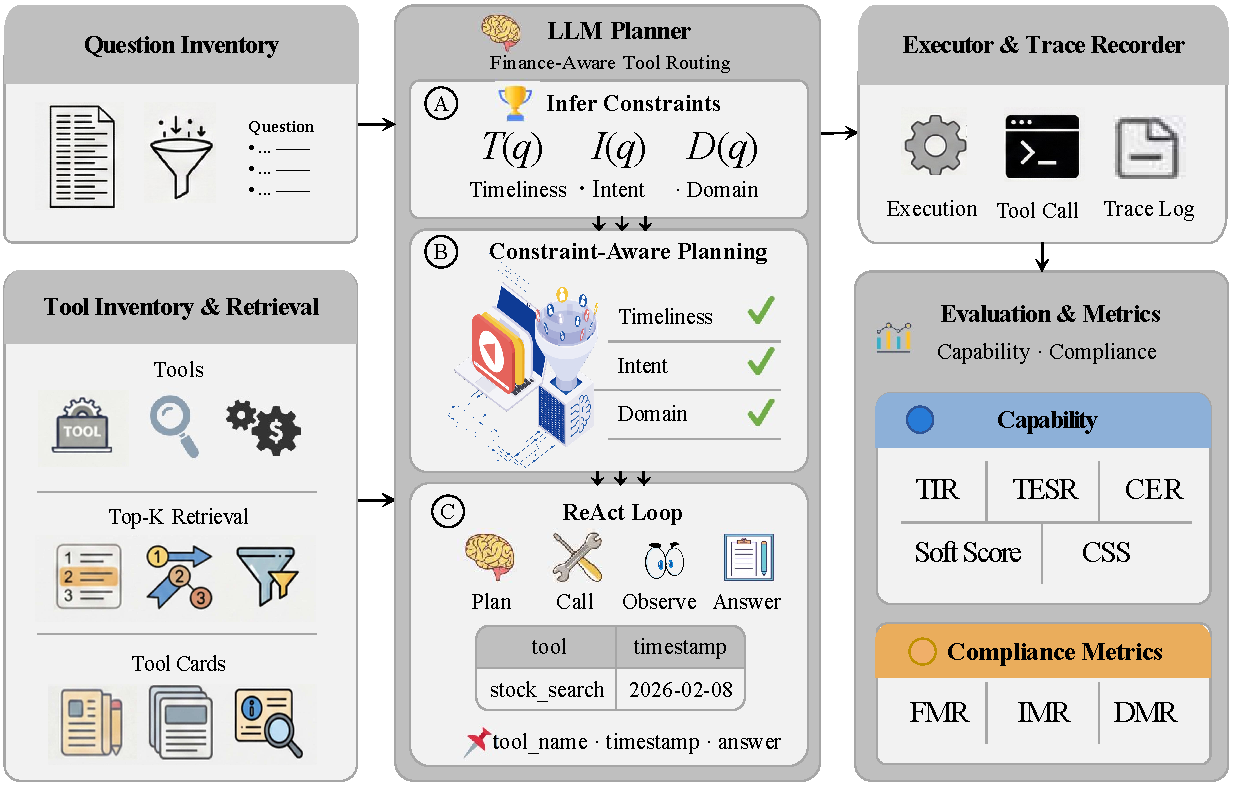
\includegraphics[width=\textwidth]{method.pdf}
\caption{Overview of Finance-Aware Tool Routing (FATR). FATR takes a Question Inventory and a Tool Inventory \& Retrieval module that performs Top-$K$ retrieval and formats retrieved tools as Tool Cards. An LLM Planner runs Finance-Aware Tool Routing by (A) Infer Constraints to derive $(T(q), I(q), D(q))$ over timeliness, intent, and domain, (B) Constraint-Aware Planning, and (C) a ReAct loop. An Executor \& Trace Recorder dispatches tool calls and trace logs, which are then scored by Evaluation \& Metrics for capability (\tir{}, \tesr{}, \cer{}, \soft{}, \css{}) and compliance (\tmr{}, \imr{}, \dmr{}).}
\Description{System overview of FATR, including question and tool inventories, Top-K retrieval and tool cards, an LLM planner that infers constraint sets T(q), I(q), and D(q) and runs a ReAct loop, and an executor with trace recording used for capability and compliance metrics.}
\label{fig:fatr}
\end{figure*}

\subsection{Problem Setup}
Let $\mathcal{T}$ denote a tool library.
Each tool $t \in \mathcal{T}$ has a callable signature $s_t$ and finance attributes $a_t=(t_t,i_t,d_t)$.
Here, $t_t$ is timeliness, $i_t$ is intent type, and $d_t$ is the set-valued regulatory domains.
Given a question $q$, an agent produces an answer $\hat{y}$ and a tool trace $\tau=\{(t_k,x_k,o_k)\}_{k=1}^{m}$.
For the $k$-th call, $x_k$ and $o_k$ denote the arguments and output.
Our executor exposes all tools through a unified interface.
The planner emits structured arguments $x_k$, and the executor validates and dispatches the call.
To support caching and evaluation, the returned output $o_k$ is normalized into a compact schema (\textit{e.g.}, key fields).

\subsection{Tool Inventory \& Retrieval and Tool Cards}
Figure~\ref{fig:fatr} summarizes the FATR pipeline end to end.
Given a question $q$ from the Question Inventory, FATR retrieves a small candidate set of tools from Tool Inventory \& Retrieval to reduce the action space.
A retriever embeds $q$ and tool metadata and selects the Top-$K$ tools by cosine similarity (default $K{=}20$) using BGE-M3 embeddings~\cite{chen2024bge}.
Each retrieved tool is formatted as a Tool Card containing tool name and description, together with the finance attributes $a_t$.
The combination reduces distractors and makes prompting more stable under large catalogs.





\subsection{Attribute-Aware Planning}
The LLM Planner runs a ReAct loop~\cite{yao2022react}: it proposes a tool call, observes tool outputs, and iterates until producing a final answer.
We cap the interaction horizon at \texttt{max\_steps{=}5} tool-augmented steps to limit latency and reduce exposure to tool drift.
During planning, FATR enforces three families of constraints derived from the question: timeliness (\textit{e.g.}, match implied time sensitivity), intent restraint (\textit{e.g.}, avoid transactional tools unless explicitly required, and in FinToolBench transactional intent is treated as disallowed and penalized), and domain alignment (\textit{e.g.}, ensure intersection between the tool domain and the inferred question domain).
% In practice, these constraints can be implemented as explicit prompt rules and, optionally, as a filter over candidate tools before execution.
In practice, these constraints are implemented as explicit prompt rules that guide the planner’s tool selection and reasoning.

Concretely, the planner first performs Infer Constraints by articulating the implied requirement sets $(T(q), I(q), D(q))$.
It then performs Constraint-Aware Planning by selecting tools whose attributes are compatible with these sets and by maintaining the constraints throughout the ReAct loop.
For multi-tool questions, the planner is encouraged to resolve ambiguity early (\textit{e.g.}, determine the correct market and ticker format) before executing downstream calls whose domains must remain consistent.
The planner is also instructed to surface key provenance fields in the final answer so that tool use is verifiable.
Figure~\ref{fig:toolcard} illustrates our tool card format, which standardizes tool metadata and exposes finance-specific attributes used for both retrieval and constraint checking.
While the primary goal is to evaluate models rather than to enforce policy, FATR can optionally apply conservative hard filters at inference time (\textit{e.g.}, excluding transactional tools and removing domain-incompatible tools) to reduce unforced compliance errors.
Pseudocode for the full pipeline is given in Appendix~\ref{sec:algorithm}.


\begin{figure}[t]
\centering
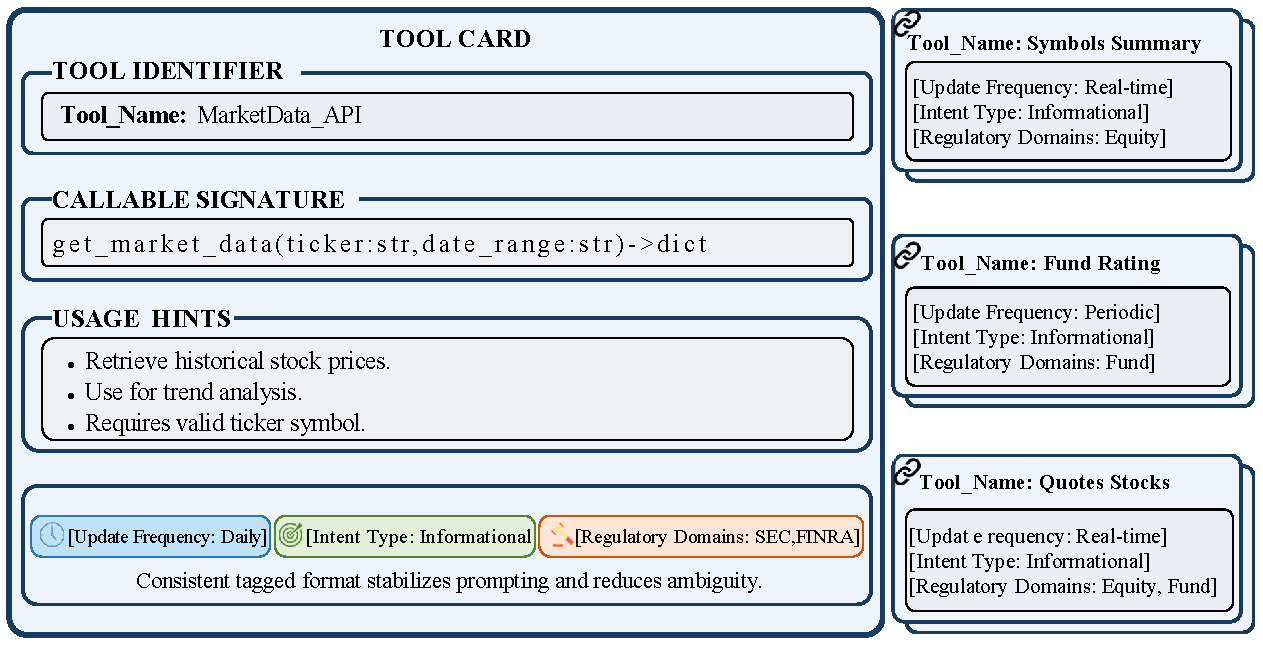
\includegraphics[width=\columnwidth]{tool_card.pdf}
\caption{Tool cards for attribute injection and constraint checking. }
\Description{Visualization of the tool card schema, with fields for tool identifier, name, callable signature, usage hints, and standardized finance tags, plus example cards for several tools.}
\label{fig:toolcard}
\end{figure}

\section{Experiments}\label{sec:experiments}

\subsection{Benchmark Setting}
The following protocol is designed so that results on FinToolBench can be reproduced and compared fairly across studies.
We run evaluation on all 295 questions.
Each run uses a fixed tool-use limit, \textit{i.e.}, at most 5 tool-use rounds per question. In each round, multiple tool calls may be issued, with a per-call timeout of 60 seconds and up to 2 retries.
Tool execution is performed in a controlled environment with deterministic caching and full logging of tool traces.
For analysis, questions are stratified by single vs multi-tool and by inferred question category. 
We report metrics following the definitions in Section~\ref{subsec:bench_metrics}.

\subsection{Baselines and Model Backends}
We evaluate FinToolBench under a unified agent framework based on FATR, which integrates tool retrieval, finance-attribute injection, and stabilized execution.
Unless otherwise specified, the overall pipeline including the retriever and executor is fixed, and only the LLM planner varies across different model backends.
We consider several representative LLM backends as planners, including Doubao-Seed-1.6, Qwen3-8B, GLM-4.7-Flash, and GPT-4o.
All models interact with the same tool inventory, retrieval results, and execution environment, ensuring that performance differences can be attributed to the planner’s reasoning and tool-selection behavior rather than infrastructure variation.
For answer correctness and requirement inference, we employ an LLM-as-a-judge.
Exact model versions, decoding parameters, and inference hyperparameters are reported in the appendix (Appendix~\ref{sec:commands}).

\subsection{Tool-Call Interface and Prompts}
All agent variants share the same tool-call interface: the planner outputs either a final answer or a structured tool invocation specifying a tool ID and arguments.
We constrain arguments to a JSON schema derived from the tool signature and return tool outputs in a normalized format.
Retrieved tools are converted into function schemas for function calling. We prepend the finance tags, \textit{i.e.}, timeliness, intent type, and regulatory domains, to the tool description.
For tool-using variants, the prompt emphasizes (i) using tools when timeliness is required, (ii) avoiding transactional actions, and (iii) explicitly checking that the selected tools' domains match the question.
When tool outputs exceed a length threshold, an LLM-based extractor compresses responses to question-relevant fields before returning them to the planner, limiting context growth across multi-step traces.
Detailed prompt templates and compression settings are given in the appendix~\ref{sec:prompt_templates} and appendix~\ref{sec:algorithm}.

\subsection{Judges and Agreement}
For computing \soft and for requirement inference in Eq.~\eqref{eq:mismatch}, we use GPT-5.1 as the judge and repeat each judgment three times to reduce variance.
For \soft, we average the three judge scores. 
For compliance evaluation, we perform a single LLM-judge decision per tool call, since the output is a discrete match/mismatch label rather than a graded score.

\section{Results}
\label{sec:results}

\begin{table*}[htbp]
\centering
\caption{Main results on FinToolBench.}
\label{tab:main_results}
\small
\begin{tabular*}{\textwidth}{@{}@{\extracolsep{\fill}}lcccccccc@{}}
\toprule
Model & \tir & \tesr & \cer$\uparrow$ & \soft$\uparrow$ & \css$\uparrow$ & \tmr$\downarrow$ & \imr$\downarrow$ & \dmr$\downarrow$ \\
\midrule
Doubao-Seed-1.6 & 0.6508 & 0.3254 & 0.5000 & 0.3958 & 0.4627 & 0.3438 & 0.6563 & 0.1719 \\
Qwen3-8B        & 0.8712 & 0.2949 & 0.3385 & 0.4234 & 0.4040 & 0.3307 & 0.6887 & 0.1673 \\
GLM-4.7-Flash   & 0.4407 & 0.2102 & 0.4769 & 0.2769 & 0.3791 & 0.4615 & 0.7231 & 0.1769 \\
GPT-4o          & 0.2267 & 0.1400 & 0.6176 & 0.2302 & 0.6700 & 0.3529 & 0.5000 & 0.1176 \\
\bottomrule
\end{tabular*}
\end{table*}

\subsection{Main Results}
Table~\ref{tab:main_results} reports the end-to-end results on FinToolBench.
A low \tir indicates a tendency to rely on parametric knowledge rather than tool invocation, while a low \cer points to planning or argument errors despite successful invocation. High mismatch rates signify that while traces may be executable, they violate specific finance constraints.
Qwen3-8B exhibits the highest tool invocation rate (\tir=0.8712) and achieves the highest soft accuracy (\soft=0.4234). However, its comparatively low \cer (0.3385) implies that while it is eager to use tools, it frequently suffers from argument instantiation errors or execution failures.
Doubao-Seed-1.6 demonstrates the most balanced performance, attaining the highest overall execution success rate (\tesr=0.3254) and the second-highest \cer (0.5000), suggesting reliable tool planning and argument construction.
GLM-4.7-Flash shows weaker performance, characterized by higher mismatch rates across all dimensions (\tmr, \imr, \dmr) and the lowest conditional success score (\css=0.3791).
Conversely, GPT-4o adopts an extremely conservative strategy with the lowest invocation rate (\tir=0.2267), leading to the lowest overall coverage (\tesr=0.1400). Yet, when it does choose to invoke tools, it is highly precise, achieving the highest \cer (0.6176) and \css (0.6700), along with the lowest intent and domain mismatch rates, which highlights a trade-off, \textit{i.e.}, GPT-4o prioritizes safety and precision over recall, often failing to attempt tool-required queries under our protocol.
Overall, these results emphasize that neither aggressive tool use (as seen in Qwen) nor high precision (as seen in GPT-4o) is sufficient on its own. Reliable execution combined with active tool selection is necessary to maximize end-to-end performance.


\begin{figure}[t]
\centering
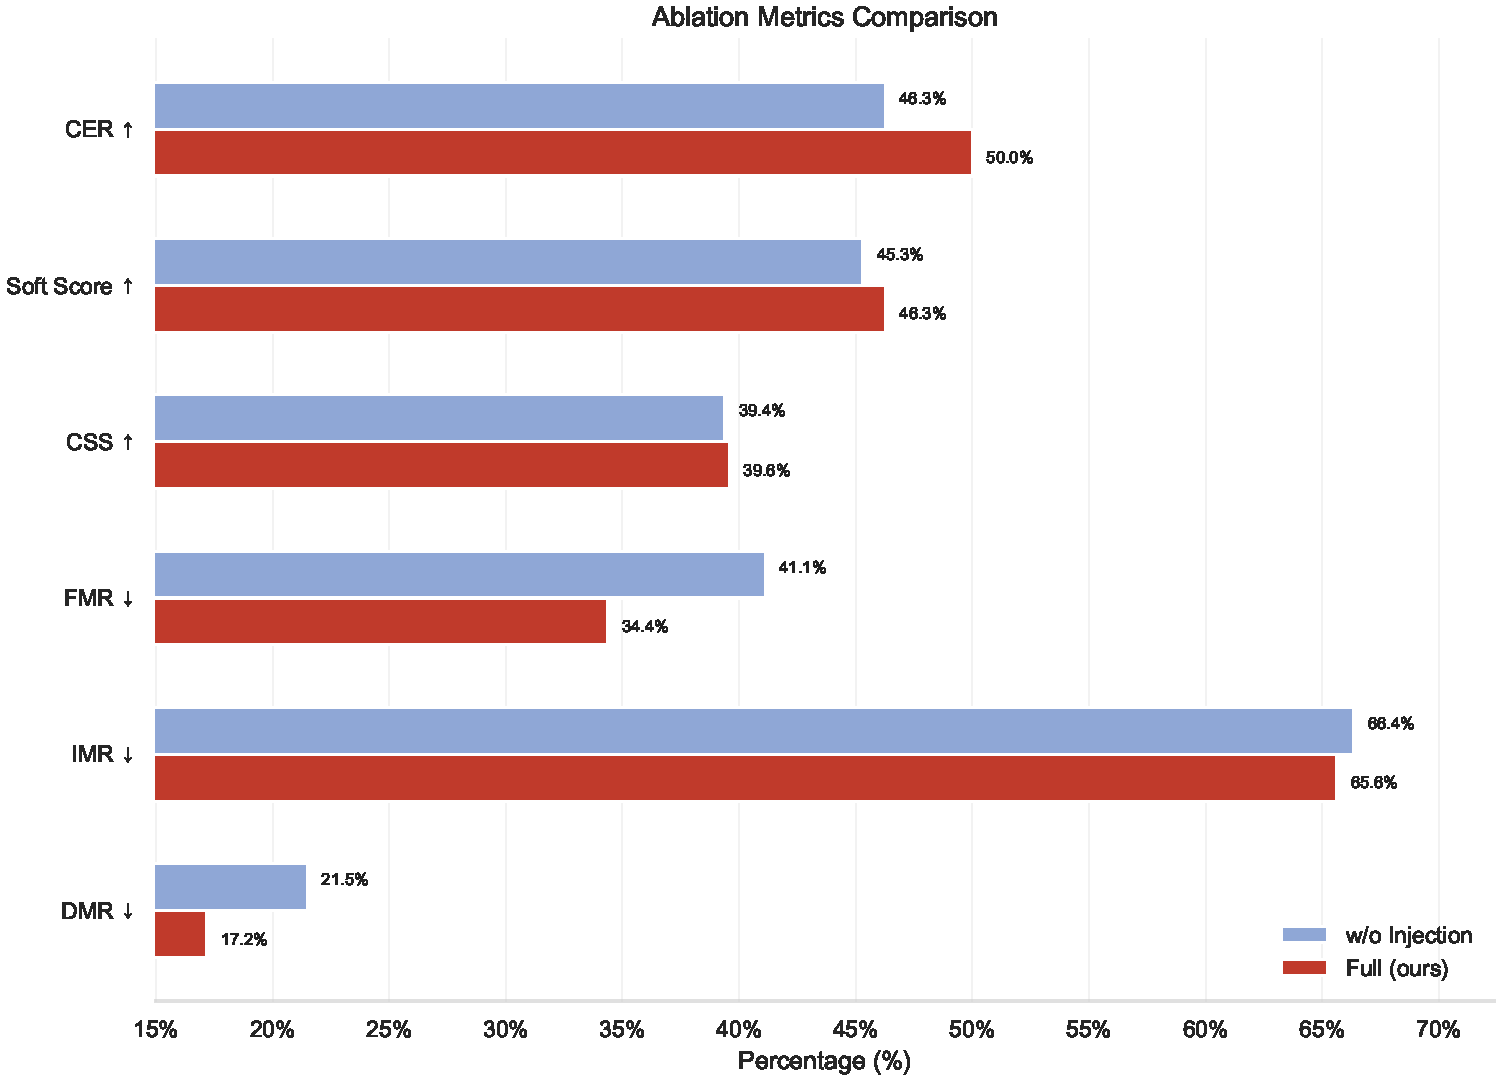
\includegraphics[width=\columnwidth]{ablation_metrics_compare.pdf}
\caption{Attribute injection ablation in \methodname{}. We compare full tool cards with finance tags against a variant without attribute injection. Injection slightly reduces tool invocation (\tir) under stricter acceptability checks, but it improves execution success conditioned on tool use (\cer) and reduces mismatch rates (\tmr{}, \imr{}, \dmr{}).}
\Description{Bar chart comparing ablation settings with and without finance attribute injection across tool-use and compliance metrics.}
\label{fig:ablation_injection}
\end{figure}



\subsection{Finance Attribute Injection}
We study whether exposing finance tags, \textit{i.e.}, timeliness, intent, and regulatory domain, inside tool cards changes tool-use behavior.
We compare full \methodname{} against a variant that keeps the same retriever and executor but omits finance tags from the tool-card text presented to the planner.
Figure~\ref{fig:ablation_injection} summarizes the resulting trade-offs between tool-use coverage, conditional execution reliability, and compliance alignment.
Two interacting effects explain the pattern.
First, adding explicit finance tags can reduce \tir because the planner is more likely to avoid marginal or risky calls when constraints are salient.
Second, \tesr can decrease mechanically because it is defined over all questions, and fewer questions enter a tool-augmented trace that can succeed.
To decouple coverage from conditional reliability, we report \cer=\tesr/\tir, which captures execution success given at least one tool call.
Overall, injection primarily improves tool choice and compliance alignment rather than executor stability.



\begin{figure}[t]
\centering
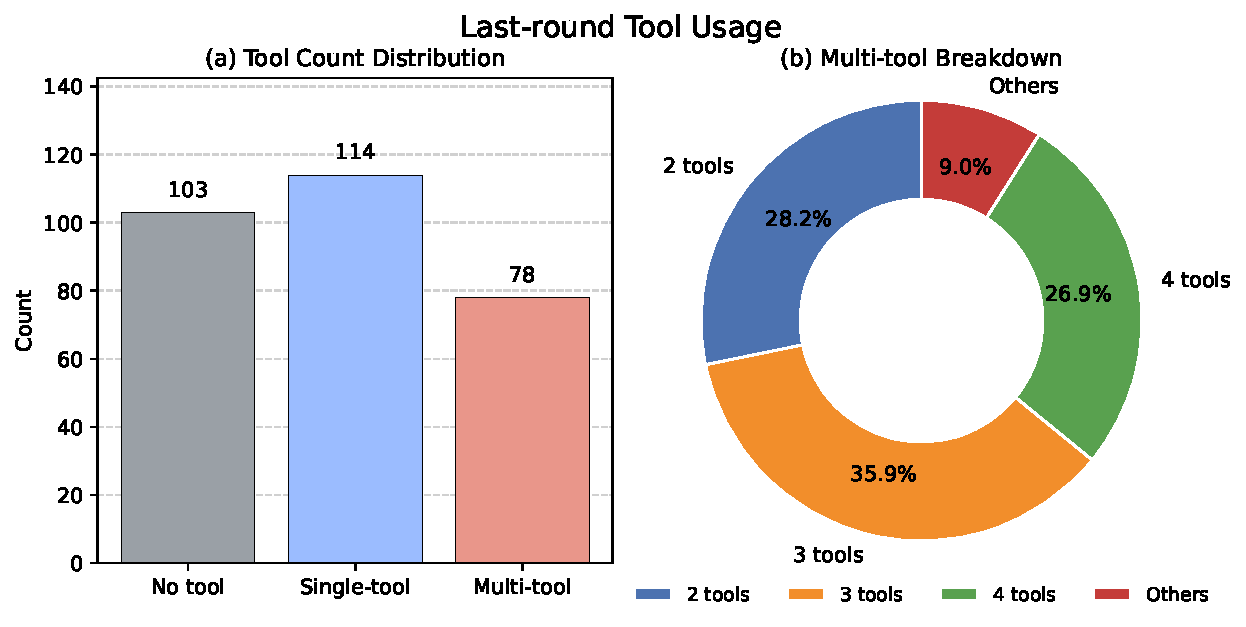
\includegraphics[width=\columnwidth]{toolcount_last_round.pdf}
\caption{Tool usage distribution on FinToolBench. Left: counts of runs with no tool call, a single tool call, and multiple tool calls. Right: breakdown of multi-tool traces by the number of tools invoked.}
\Description{A bar chart showing counts of runs by tool usage (no tool, single-tool, multi-tool) and a donut chart showing the distribution of the number of tools invoked among multi-tool traces.}
\label{fig:toolcount_last_round}
\end{figure}


\subsection{Tool Usage Distribution}
Figure~\ref{fig:toolcount_last_round} provides a complementary view by summarizing tool usage in the last-round evaluation logs of Doubao-Seed-1.6, with one run per question.
Out of 295 questions, 103 runs end without any tool call, 114 produce a single-tool trace, and 78 require multiple tools.
Among the multi-tool traces, three-tool traces are most common, followed by two- and four-tool traces.
The observed distribution motivates reporting both coverage (\tir) and conditional reliability (\cer) rather than relying on a single end-to-end success metric.

\subsection{Category-Level Diagnosis}
Aggregate metrics often mask the specific contexts in which an agent succeeds or fails. To facilitate a more granular diagnosis, we present a category-level breakdown of both capability and compliance metrics. The analysis reveals significant performance heterogeneity across tool scopes. For instance, while the agent demonstrates robustness in macro interpretation, it struggles with strict adherence in structural tasks like value extraction, despite maintaining high soft scores. Such a breakdown allows us to pinpoint whether failures stem from capability deficits or rigid formatting mismatches, as detailed in Appendix~\ref{sec:category_diagnosis}.

\section{Conclusion}
We present FinToolBench, a comprehensive framework that frames financial tool-use evaluation around both call-level capability and strict regulatory compliance.
The benchmark uniquely couples a massive free-tier tool catalog (760 tools) with 295 complex, tool-required questions. 
Crucially, our evaluation protocol separates capability metrics (whether an agent can invoke and execute tools) from compliance metrics (whether its tool choices satisfy timeliness, intent, and domain constraints), mirroring real-world requirements in financial settings.
To facilitate immediate adoption, we also provide FATR, a practical baseline that effectively operationalizes these constraints via attribute injection and stability-oriented execution wrappers.
We will open-source the tool manifest, question set, and evaluation scripts, allowing the community to standardize assessment on a common, runnable benchmark and compare agents under consistent conditions.
Future work may extend coverage to proprietary real-time data feeds and further study agent robustness under inevitable tool API updates and policy drift.

\section*{Artifact Availability}
The implementation and experimental scripts are available at:
\url{https://github.com/Double-wk/FinToolBench.git}.

\balance
\bibliographystyle{ACM-Reference-Format}
\bibliography{kdd}

\clearpage
\appendix


%=============================================================================
\section{Tool Curation Criteria}
\label{sec:tool_curation}
%=============================================================================

This section spells out the criteria used to build the \bench{} tool inventory.
The pipeline retains only tools that are executable under free-tier constraints.

\subsection{RapidAPI Endpoints}

Our RapidAPI pool is initialized from finance-related tools collected from the ToolBench paper, and then filtered with the two-stage pipeline below.

\paragraph{First-stage (rule-based) filters.}
Because RapidAPI listings vary in how authentication, billing, and rate limits are described, we programmatically crawl and parse endpoint pages to extract these fields, and then apply the deterministic criteria in Table~\ref{tab:rapidapi_filters}. An endpoint is excluded if it fails any row.


\begin{table}[h]
\centering
\caption{First-stage RapidAPI filter criteria.}
\label{tab:rapidapi_filters}
\small
\begin{tabular*}{\columnwidth}{@{}@{\extracolsep{\fill}}p{0.22\linewidth}p{0.72\linewidth}@{}}
\toprule
Criterion & Rule \\
\midrule
Description & Missing or empty $\rightarrow$ excluded. \\
Deduplication & Duplicate names: keep first only. \\
Authentication & Exclude if \texttt{Authorization} or multi-step token (beyond single API key) required. \\
Existence & Remove if endpoint does not resolve or returns persistent errors. \\
Bank-card & Exclude if free-tier requires card binding. \\
Rate limits & Require $\ge$10/h, $\ge$100/d, $\ge$300/m. \\
Map & Use an LLM to align endpoint parameter names with the tool signature and then manually spot-check the mappings. \\
\bottomrule
\end{tabular*}
\end{table}

\paragraph{Second-stage (mapping and executability).}
Each endpoint that passes the first stage is mapped into our normalized schema.
We align its parameter names to our tool signature with an LLM and then manually spot-check the mappings.
We then test each mapped endpoint with at least one successful invocation (valid request and parsed response).
Endpoints that fail consistently (timeouts, validation errors, or empty responses) are dropped.

\paragraph{Outcome.}
After the two-stage filtering process, we obtain 261 executable RapidAPI endpoints.
All retained endpoints have at least one documented required or optional parameter.
Endpoints that are parameter-free or rely solely on implicit path/query conventions are excluded.


\subsection{AkShare Interfaces}

AkShare functions are selected and then validated for executability.

\paragraph{Finance-domain filter.}
Function names are matched against a fixed set of finance-related keywords.
A function is retained if its name (or module path) contains any of the following tokens:
\begin{itemize}[leftmargin=*,nosep]
\item \texttt{stock}, \texttt{fund}, \texttt{bond}, \texttt{futures}, \texttt{option}, \texttt{index}, \texttt{macro}, \texttt{currency}, \texttt{fx}, \texttt{crypto}, \texttt{rate}, \texttt{treasury}, \texttt{etf}
\item \texttt{finance}, \texttt{bank}, \texttt{insurance}, \texttt{security}, \texttt{derivative}, \texttt{swap}, \texttt{gold}, \texttt{commodity}, \texttt{interest}, \texttt{libor}, \texttt{shibor}, \texttt{exchange}, \texttt{margin}
\end{itemize}

\paragraph{Executability.}
Each candidate is invoked with minimal valid arguments, using defaults or small example values where possible.
Interfaces that raise import errors, signature errors, or runtime errors under a timeout are discarded.

\paragraph{Outcome.}
After finance-domain filtering and executability validation, we retain 499 AkShare interfaces in the final tool inventory.

\subsection{Combined Inventory}

After executability filtering, the final tool library contains 760 tools.
All tools in \bench{} are normalized into a single manifest schema, including tool name, description, and parameters.
This unified manifest enables auditable tool traces and call-level compliance metrics (TMR, IMR, DMR), where each run records the invoked tools together with their arguments and execution outcomes.


%=============================================================================
\section{Finance Attribute Schema and Labeling}
\label{sec:attributes}
%=============================================================================

Each tool is annotated with finance attributes that make timeliness, intent, and domain constraints explicit.
These attributes support both tool cards (for planning) and compliance evaluation (TMR, IMR, DMR).

\subsection{Attributes of the Tools}

\begin{itemize}[leftmargin=*]
\item \textbf{Timeliness} (\texttt{timeliness}): one of\\
  \realt, \dailyt, \asfiledt, \periodict, or \statict.
  \begin{itemize}[nosep]
  \item \realt: intra-day, low latency, such as ticks and order book.
  \item \dailyt: updated once per trading day or batch, such as closing prices and NAV.
  \item \asfiledt: event-driven, when a regulated entity files, such as filings and announcements.
  \item \periodict: fixed calendar schedule, such as quarterly reports and GDP.
  \item \statict: rarely changes, such as identifiers and listing dates.
  \end{itemize}
\item \textbf{Intent type} (\texttt{intent\_\allowbreak type}): one of\\
  \informational, \advisory, or \transactional.
  \begin{itemize}[nosep]
  \item \informational: read-only data access and factual retrieval without recommendations or actions.
  \item \advisory: analysis or recommendation-oriented outputs that go beyond pure retrieval.
  \item \transactional: action-triggering operations such as order placement, transfer, or account-changing behavior.
  \end{itemize}
\item \textbf{Regulatory domain} (\texttt{regulatory\_\allowbreak domain}):\newline
  Subset of \{equity, bond, fund, forex, derivatives, macro,\\ economic\_\allowbreak policy, sentiment\_\allowbreak trading, esg, crypto\}. Multiple values are allowed per tool.
\end{itemize}

\subsection{Labeling Protocol}

Annotations are produced by an LLM (Qwen3-8B) given the tool name and description.
Each attribute is labeled independently with three samples, and the final label is the majority vote.
This protocol keeps labeling separate from the agent under test and makes the compliance layer auditable.

%=============================================================================
\section{Question Set Construction}
\label{sec:questions}
%=============================================================================

The question set is built so that every retained question requires tool use.
Questions answerable by static memorization or general reasoning are excluded.

\subsection{Sources}

Questions are drawn from the FinanceBench release and the OpenFinData release (dataset identifier \texttt{openfindata\_}\allowbreak\texttt{release}).
Only questions that require tool calls to answer are retained, such as current prices, time series, or structured data.

\subsection{Filters}

\begin{itemize}[leftmargin=*,nosep]
\item \textbf{Standardization:} Convert all sources into a unified \texttt{\{question, answer, category\}} format.
\item \textbf{Maximum length:} 500 characters to keep prompts within a fixed budget.
\item \textbf{Candidate retrieval:} For each question, retrieve Top-$K$ tools ($K{=}20$) using BGE-M3 embeddings.
\item \textbf{LLM tool selection:} Given the Top-$K$ tools, Qwen3-8B selects the most suitable tool(s). We sample three times and keep tools with at least two votes.
\item \textbf{Deduplication:} For single-tool questions, keep at most two questions per tool to reduce skew. Multi-tool questions are not deduplicated by tool set.
\end{itemize}

\subsection{Outcome}

The final question set contains 295 questions, spanning both simple and compositional tool use: 166 single-tool questions and 129 multi-tool questions, classified by the number of tool calls observed at runtime.

%=============================================================================
\section{Metric Definitions}
\label{sec:metrics}
%=============================================================================

All metrics are defined over a fixed question set and a fixed evaluation protocol (timeout, retries, caching).
We report capability (TIR, TESR, CER) and compliance (TMR, IMR, DMR) to separate whether an agent can run tools from whether its tool choices satisfy finance constraints.
Below, $N$ denotes the number of questions.

\subsection{Capability}

\begin{itemize}[leftmargin=*]
\item \textbf{Tool Invocation Rate (\tir).} Fraction of questions whose execution invokes at least one tool call:
\[\mathrm{TIR}=\frac{1}{N}\sum_{i=1}^{N}\mathbf{1}\!\left[\,|\mathrm{tool\_calls}_i|>0\,\right].\]
\item \textbf{Tool Execution Success Rate (\tesr).} Fraction of questions whose tool execution succeeds.
We mark a question successful when its final tool call returns a valid parsed output without error or exception; intermediate failures and retries are allowed:
  \[\mathrm{TESR}=\frac{1}{N}\sum_{i=1}^{N}\mathbf{1}\!\left[\,\text{final tool call succeeds on question } i\,\right].\]
\item \textbf{Conditional Execution Rate (\cer).} Success rate among questions that invoked at least one tool call: 
  \[\mathrm{CER}=\frac{\mathrm{TESR}}{\mathrm{TIR}},\quad \mathrm{CER}=0 \text{ when } \mathrm{TIR}=0.\]
\item \textbf{Soft Score (\soft).} 
We partition questions into three types based on the gold-answer format:
(i) numeric/choice questions, identified by the presence of a \texttt{numeric} or \texttt{choices} field in the gold answer;
(ii) structured-analysis questions, identified by the presence of a \texttt{criterium} field in the gold answer;
(iii) \texttt{other} questions, all remaining non-numeric/choice/\texttt{criterium} cases.
All questions are judged by LLM (GPT-5.1). Numeric/choice questions are scored in $\{1,0\}$, while structured-analysis and \texttt{other} questions are scored in $\{1,0.5,0\}$. Scores are averaged over three judging repeats.
\[\mathrm{SoftScore}=\frac{1}{3N}\sum_{i=1}^{N}\sum_{r=1}^{3} s_{i,r}.\]
\item \textbf{Conditional Soft Score (\css).} Mean \soft{} over questions with successful execution:
  \[\mathrm{CSS}=\frac{\mathrm{Soft\ Score}}{\mathrm{TESR}},\quad \mathrm{CSS}=0 \text{ when } \mathrm{TESR}=0.\]
\end{itemize}



\subsection{Compliance Mismatch Rates}

For each question $q$, an LLM(GPT-5.1) judge assesses whether the tools used in the execution are aligned with the question's finance constraints in timeliness, intent type, and regulatory domain.
Let the executed tool-use trace be $\tau=\{(t_k,x_k,o_k)\}_{k=1}^{m}$, where $t_k$ is the tool name selected at step $k$, $x_k$ is the tool input (arguments), and $o_k$ is the tool output.
Tool attributes are not part of the trace; instead, for any tool $t$ we look up its finance tags from the tool metadata:
$A(t)=(t(t), i(t), d(t))$, corresponding to timeliness $t(t)$, intent type $i(t)$, and regulatory domains $d(t)$.

Define judge-level call alignment indicators:
$J_T(q,t_k,x_k,o_k,T(t_k))\in\{0,1\}$,
$J_I(q,t_k,x_k,o_k,I(t_k))\in\{0,1\}$,
and $J_D(q,t_k,x_k,o_k,D(t_k))\in\{0,1\}$,
where $1$ means matched and $0$ means mismatched.
We then define mismatch-at-least-once indicators at the question level:
\begin{align*}
\mathrm{TMR}(q,\tau) &= \mathbf{1}\!\left[\exists k:\ J_T(q,t_k,x_k,o_k,T(t_k))=0\right], \\
\mathrm{IMR}(q,\tau) &= \mathbf{1}\!\left[\exists k:\ J_I(q,t_k,x_k,o_k,I(t_k))=0\right], \\
\mathrm{DMR}(q,\tau) &= \mathbf{1}\!\left[\exists k:\ J_D(q,t_k,x_k,o_k,D(t_k))=0\right].
\end{align*}

TMR, IMR, and DMR count the number of questions whose traces contain at least one mismatched tool call in the corresponding dimension.
Each question is counted once, regardless of how many mismatches occur in its trace.
We report these metrics as rates in $[0,1]$ by dividing the mismatch count by the number of questions that invoked at least one tool call.
Lower is better.



%=============================================================================
\section{Prompt Templates}
\label{sec:prompt_templates}
%=============================================================================

This section documents the prompts for (i) intent mismatch evaluation, (ii) planner system instructions, and (iii) RapidAPI Parameter Alignment.

\subsection{Intent-Match Evaluator (IMR)}

We use an LLM(GPT-5.1) judge to decide whether a tool call's \texttt{intent\_type} is compatible with the question requirement.
The judge considers only intent (informational, advisory, transactional) and ignores execution success.

\begin{promptcard}{Intent match prompt (JSON-only output)}
You are a financial tool compliance evaluator. Determine whether the "question requirement" matches the "tool intent".\\
Consider only tool intent. Do not consider whether the tool call succeeds.\\
Tool intent must be one of \texttt{informational} / \texttt{advisory} / \texttt{transactional}.

Question: \{question\}\\
Tool name: \{tool\_name\}\\
Tool intent (\texttt{intent\_type}): \{tags.get("intent\_type")\}\\
Tool description: \{tags.get("description") or ""\}

Output JSON only:
\{
  "match": "yes|no",
  "reason": "within 20 words"
\}
\end{promptcard}

\subsection{Planner System}

The planner is explicitly instructed to use the \texttt{financial\_tags} field inside each tool description when choosing tools.
This makes timeliness, domain, and intent cues salient at selection time.

\begin{promptcard}{Planner system}
% You can see the \texttt{financial\_tags} field in tool descriptions.\\
% When selecting tools, use these attributes to help your decision, including the tool's timeliness, regulatory domain, and compliance risk.\\
% Subject to satisfying the question, prefer tools with appropriate timeliness whose domain and intent better match the requirement.
Subject to satisfying the question, first infer the question’s required finance tags:
(a) required \texttt{timeliness}, (b) required \texttt{regulatory\_domains}, and (c) allowed \texttt{intent\_type}.\\
Then select tools whose \texttt{financial\_tags} best match these requirements: require domain overlap, prefer matching timeliness, and choose the lowest-risk intent (\texttt{informational} > \texttt{advisory}; avoid \texttt{transactional} unless explicitly requested).\\
If multiple tools match, choose the one whose signature/description best fits the needed inputs/outputs.
\end{promptcard}

\subsection{RapidAPI Parameter Alignment}

RapidAPI documentation often uses parameter names that differ from those used in request examples.
To reduce argument instantiation errors, we generate normalized Python wrappers whose function parameters exactly match the keys used in the request schema, and we verify mappings with manual spot-checking (Table~\ref{tab:rapidapi_filters}, Map rule).
For security, we show the API key as a placeholder.

\begin{promptcard}{Parameter-aligned Python code generation prompt}
You are a professional Python tool function generator. Rewrite the following raw API call code into a standard reusable function.\\
Strictly follow the rules below.\par

1. Function name: \{func\_name\}\\
2. Function parameters:\par
- All input parameters: \{param\_str\}\\
- Additional fixed parameter: \texttt{rapidapi\_key: str = "<RAPIDAPI\_KEY>"}\par
3. The function must:\par
- Use \texttt{requests} to send the HTTP request\\
- Use \texttt{X-RapidAPI-Key} and \texttt{X-RapidAPI-Host} in headers\\
- Return \texttt{response.json()} if possible, otherwise return \texttt{response.text}\\
% - Do not use \texttt{print}. Always \texttt{return}\\
% - Include a full docstring describing the function and every parameter\\
- Do not explain anything. Output pure Python code only\\
- Parameter names must exactly match the keys in the parameter dictionary (case sensitive)\par

Description: \{desc\}\\
Parameter spec: \{parameters\}\par
URL:\{url\}\par
X-RapidAPI-Host:\{url.split('/')[2]\}\par

\end{promptcard}


%=============================================================================
\section{Commands and Reproduction Checklist}
\label{sec:commands}
%=============================================================================

The following enables independent reproduction of the benchmark and evaluation pipeline so that results can be compared fairly across studies.

\subsection{Environment and Models}

RapidAPI keys are obtained following the official documentation. AkShare usage follows its documentation.
Retriever: BGE-M3. Planner: exact model names and versions, for example Doubao-Seed-1.6, Qwen3-8B, and GLM-4.7-Flash, plus inference hyperparameters (temperature, max tokens).
Judge: GPT-5.1 (3 repeats) for \soft{} and requirement metrics. Record these identifiers in the repository \texttt{README} or a config file so that tables in the paper can be reproduced.

%=============================================================================

\section{Algorithm --- FATR Pipeline}
\label{sec:algorithm}
%=============================================================================

\begin{algorithm}[H]
\caption{FATR pipeline}
\begin{algorithmic}[1]
\Require Question $q$, tool library $\mathcal{T}$, retriever $\mathcal{R}$, planner LLM $\pi$, Top-$K$ (default $K{=}20$)
\Ensure Final answer $\hat{y}$, tool trace $\tau$
\State $\mathcal{C} \gets \mathcal{R}(q, \mathcal{T}, K)$ \Comment{Retrieve Top-$K$ tools by similarity}
\State Build tool cards: for each $t \in \mathcal{C}$, format $\mathrm{Card}(t)$ with signature and finance attributes
\State $\tau \gets \emptyset$, $h \gets \emptyset$ \Comment{History of tool calls and outputs}
\Repeat
\State Planner $\pi$ proposes next action given $(q,\{\mathrm{Card}(t)\}_{t\in\mathcal{C}},h)$: tool $t$ and arguments $x$ (or final answer $\hat{y}$)
\If{action is tool call $(t, x)$}
\State Validate $t \in \mathcal{C}$
\State Execute: $o \gets \mathsf{Exec}(t, x)$ with timeout, optionally compress $o$
\State Append $(t, x, o)$ to $\tau$, update $h$ with observation
\Else
\State $\hat{y} \gets$ planner output, \textbf{break}
\EndIf
\Until{planner emits final answer or max steps}
\State \Return $\hat{y}$, $\tau$
\end{algorithmic}
\end{algorithm}
\FloatBarrier



The algorithm in this section summarizes the \methodname{} pipeline: retrieval, tool-card formatting, ReAct-style planning with finance constraints, and stabilized execution (timeout, retries, cache, optional output compression).
When output compression is enabled, we use Qwen3-8B as the extractor to keep only question-relevant fields from long tool responses.
This algorithm serves as the reference implementation for the \methodname{} baseline in the main paper.

% Attribute injection ablation is reported in the main paper (Section~\ref{sec:experiments}).

%============================================================================
\section{Category-Level Diagnosis}
\label{sec:category_diagnosis}
%=============================================================================

To further localize failure modes beyond aggregate averages, we report metrics broken down by question category.
Figure~\ref{fig:metrics_by_category} presents category-level performance for Doubao-Seed-1.6.
The heatmap highlights substantial heterogeneity across categories.
Categories with low \tir cap end-to-end execution success by limiting tool coverage.
In contrast, categories with high \tir but low \tesr indicate difficulties in argument construction, disambiguation, or endpoint instability even after the agent commits to tool use.

\begin{figure*}[!tb]
\centering
% 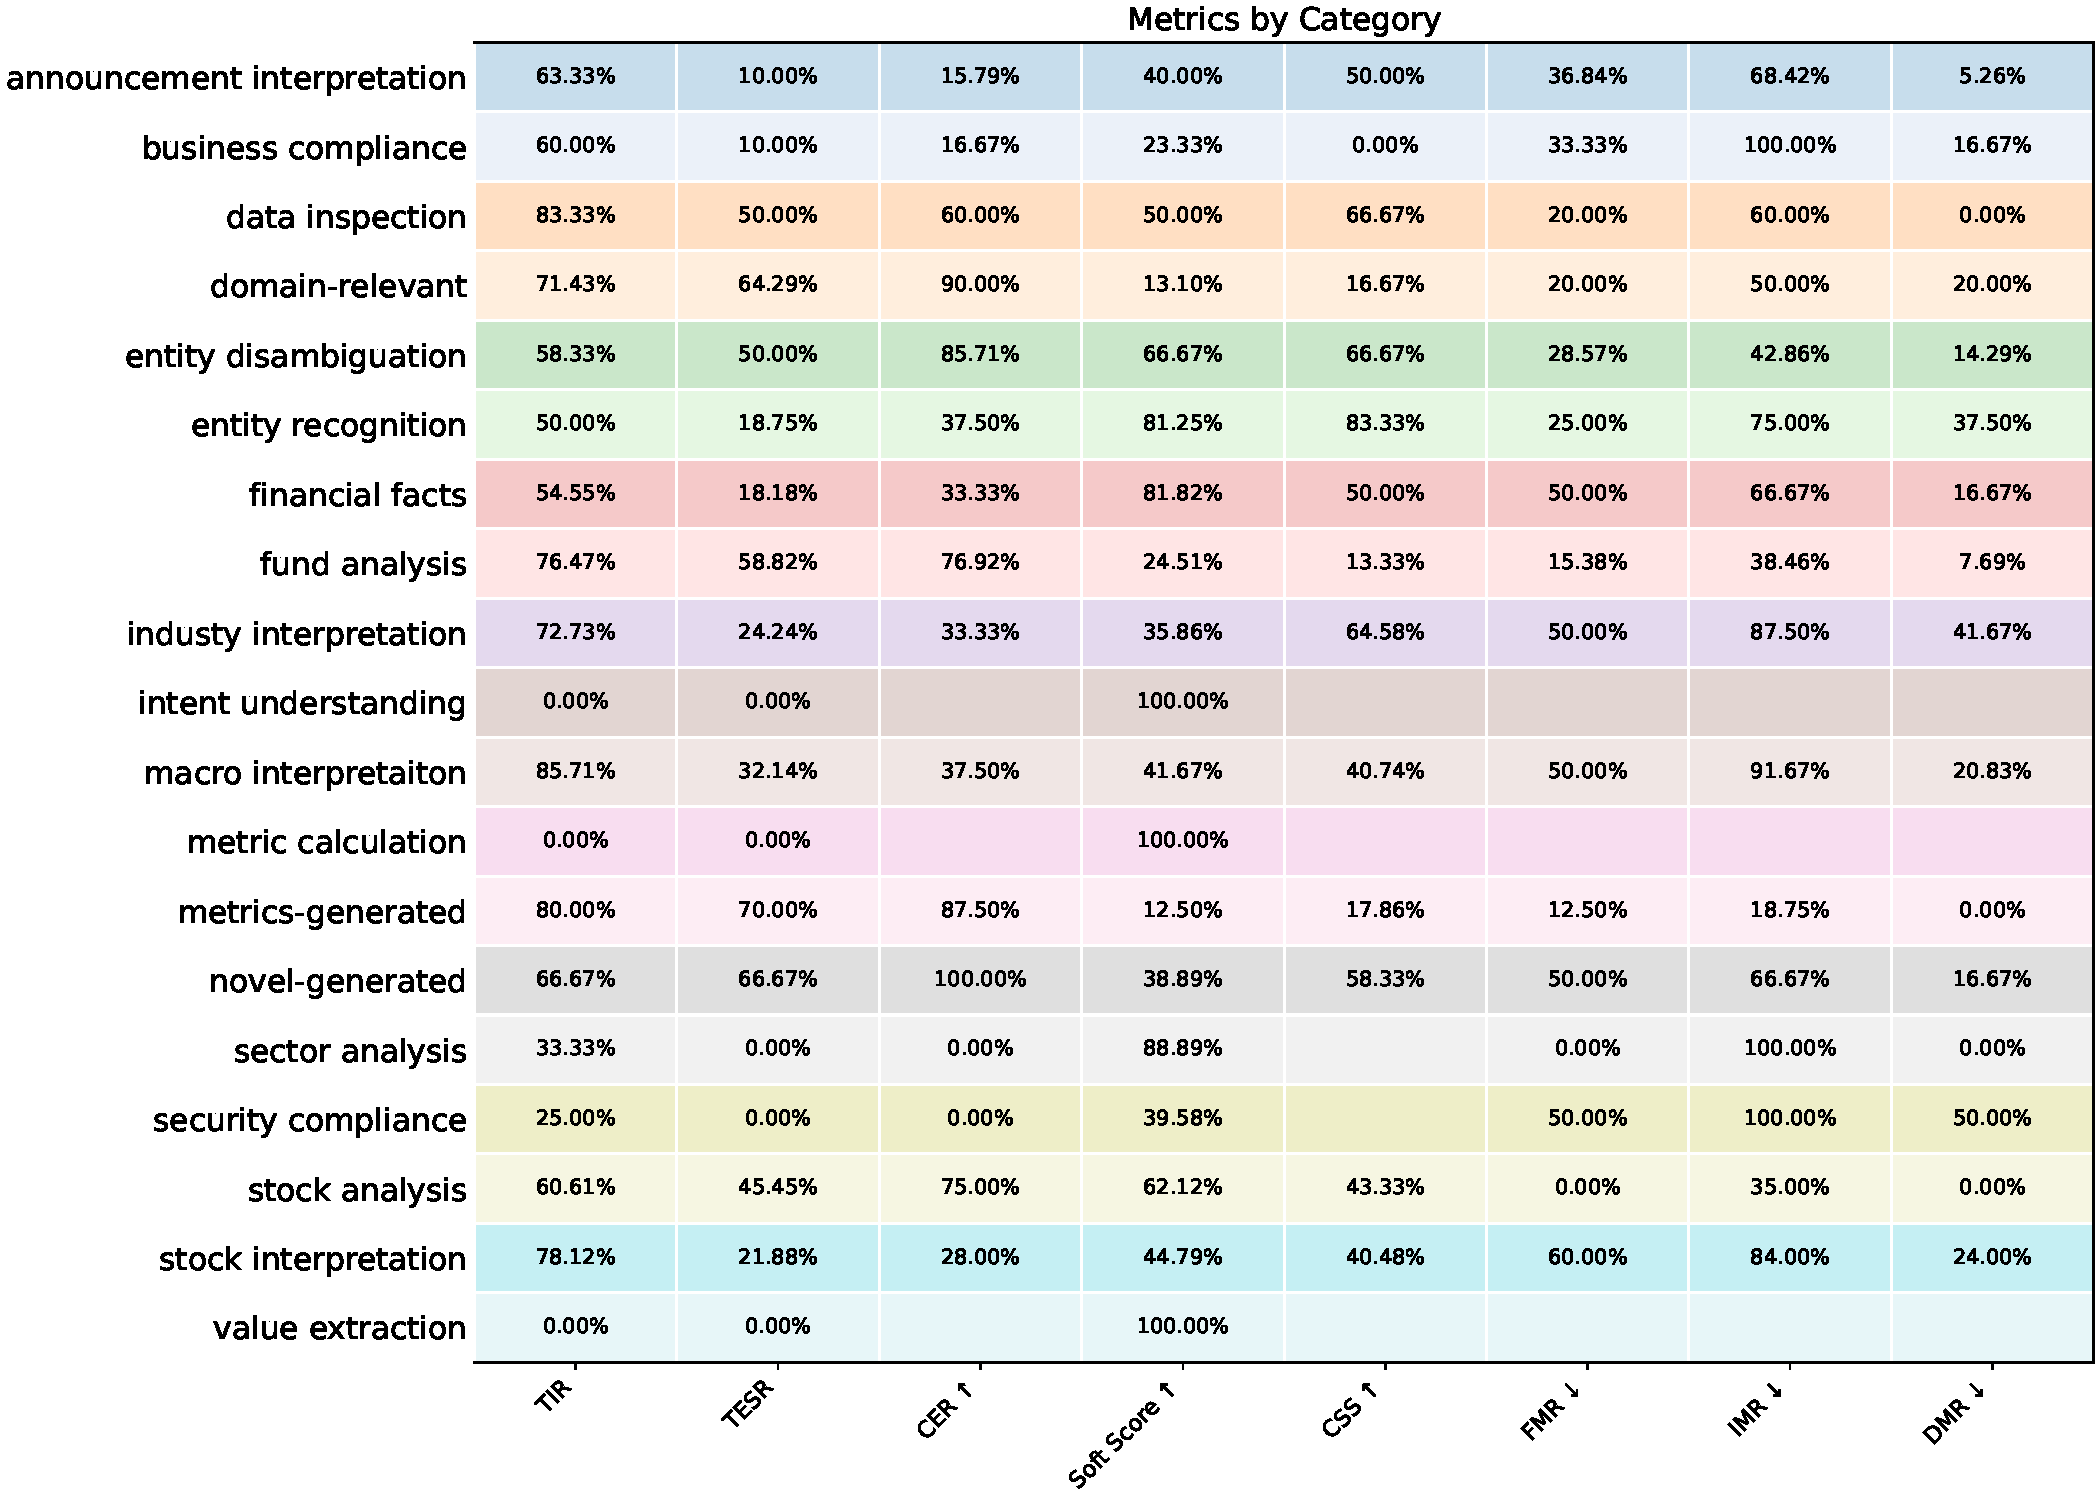
\includegraphics[width=\textwidth]{result_Doubao-Seed-1.6_full_by_category.pdf}
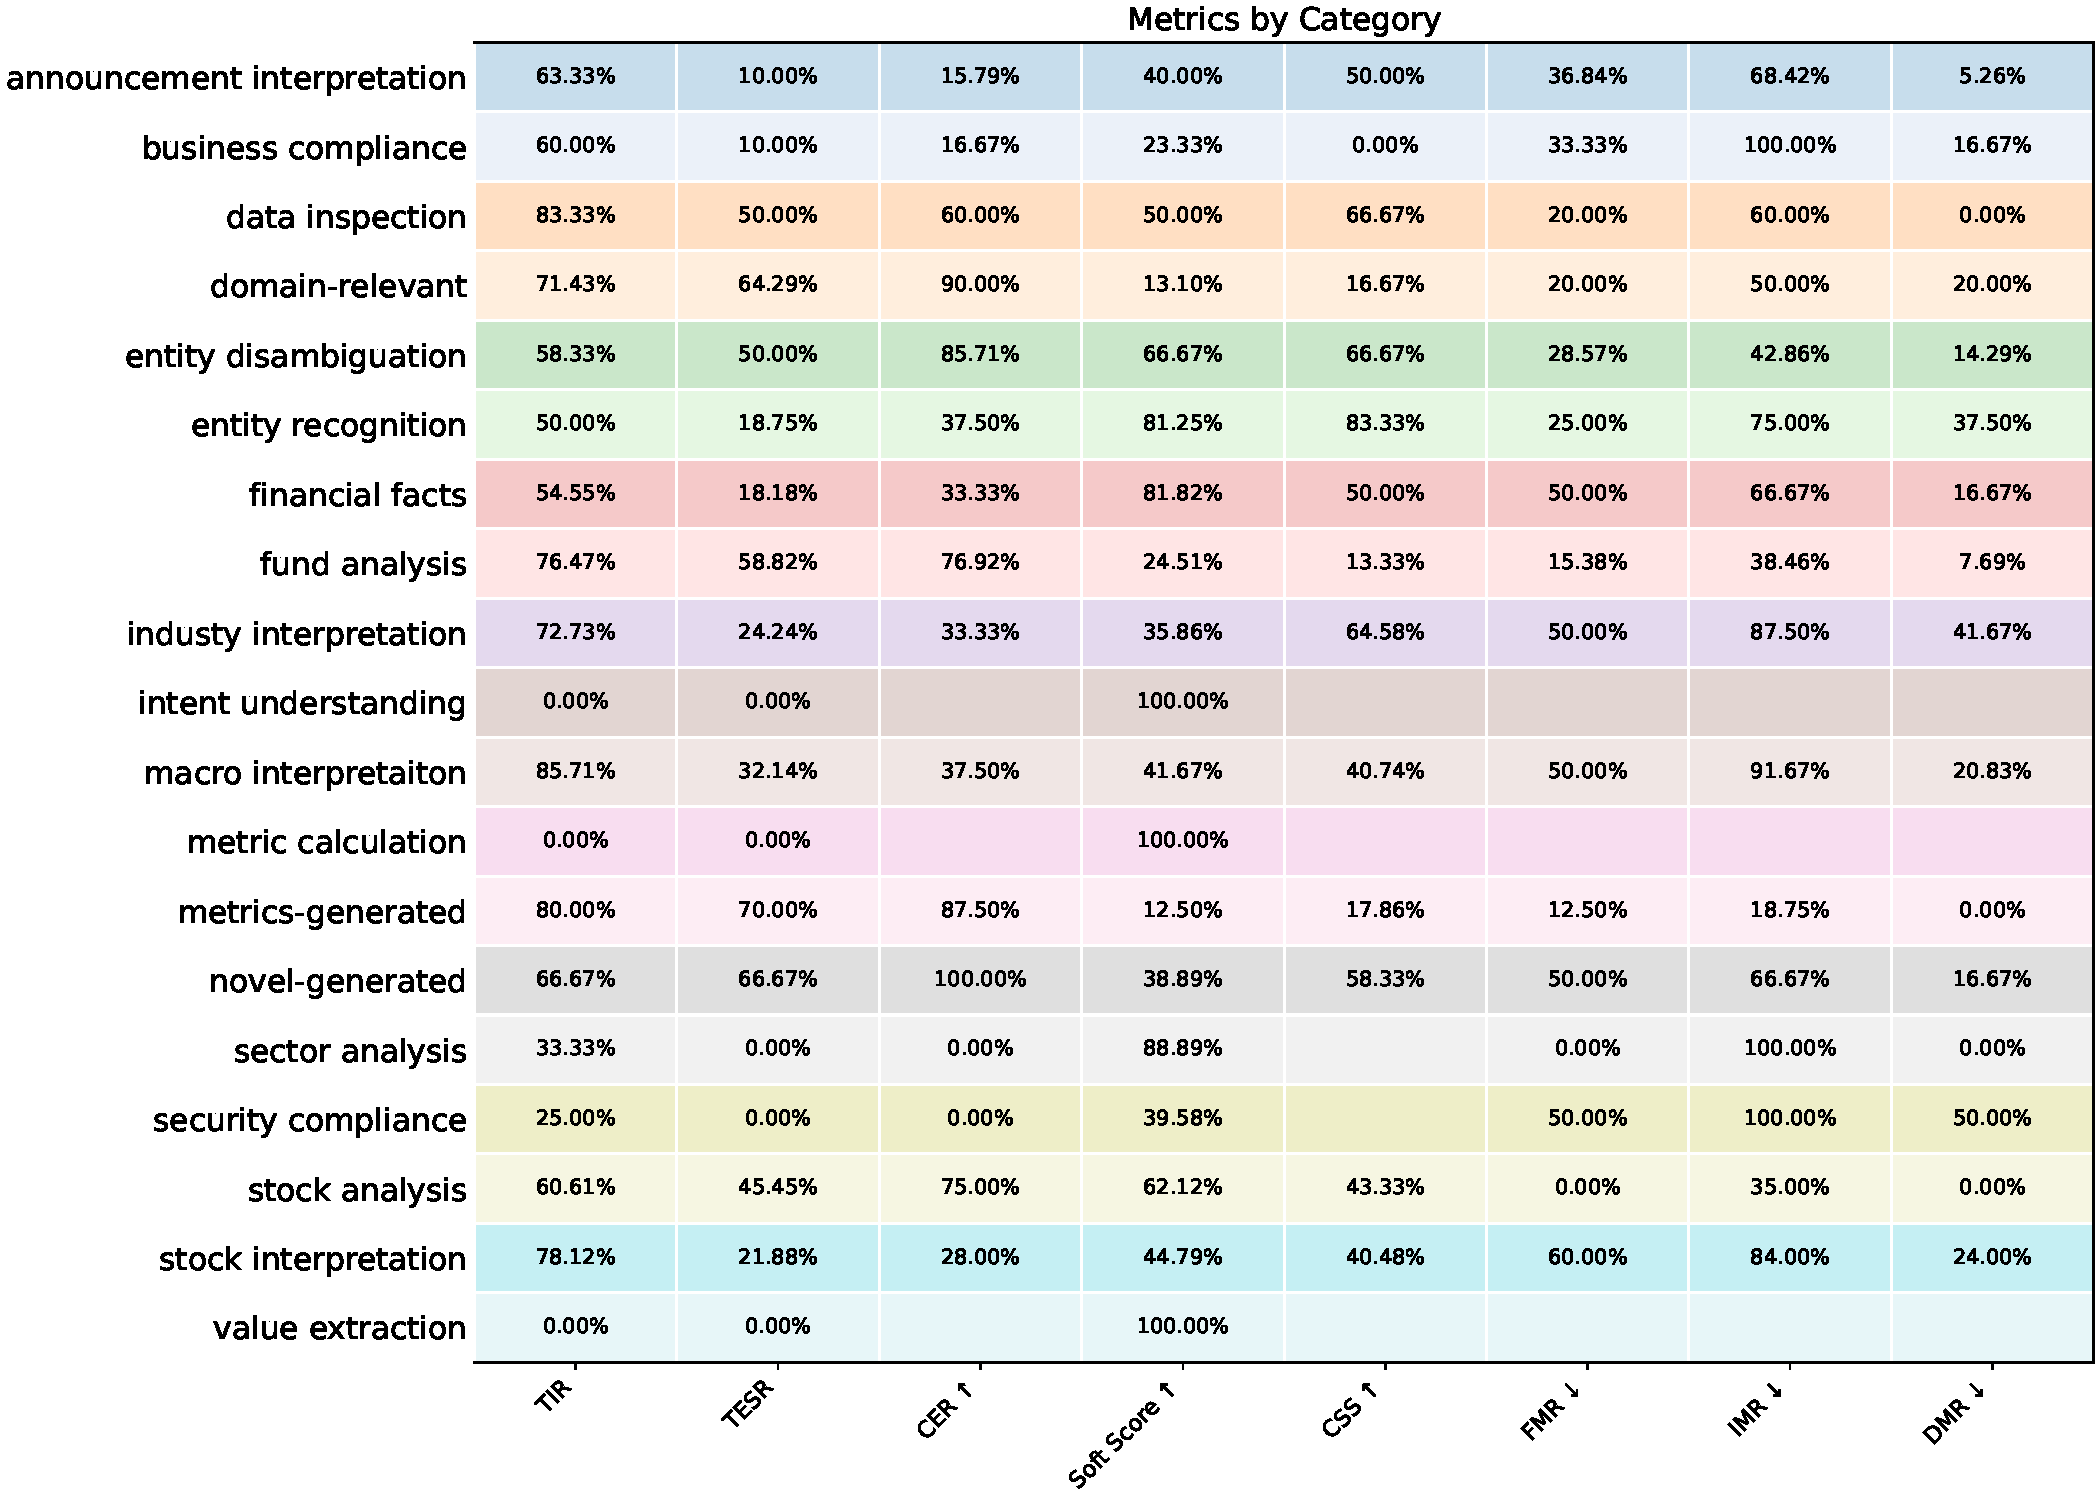
\includegraphics[scale=0.38]{result_Doubao-Seed-1.6_full_by_category.pdf}
\caption{Metrics by category for Doubao-Seed-1.6 on FinToolBench. Rows are question categories and columns are evaluation metrics.}
\Description{Heatmap of FinToolBench metrics by category for Doubao-Seed-1.6.}
\label{fig:metrics_by_category}
\end{figure*}

%=============================================================================



%=============================================================================
\section{Case Studies}
\label{sec:case_studies}
%=============================================================================

This section presents representative end-to-end execution traces from our evaluation logs.
Each case study reports the full question, the agent's tool calls (with condensed outputs),
the final answer, correctness against dataset ground truth, and an analysis highlighting
what the trace reveals about agentic financial tool use.

%=============================================================================
\subsection{Case Study 1: Finance Attribute Injection Changes Tooling Behavior}
\label{sec:case_study_financebench_margin}
%=============================================================================

This case examines whether finance-attribute injection changes tool-selection behavior
when the first attempted interface is partially incompatible with the benchmark wrapper.
We compare a baseline planner (without attribute tags in tool cards) against \methodname{}
under the same retrieval pool and execution budget. The key question is not only whether
the run finishes, but whether the resulting trace supports the dataset's intended reasoning target.

\begin{figure*}[htbp]
\begin{casecard}{Case Study 1 (\texttt{financebench\_9}): injection recovers tool execution but not task framing}
\textbf{Question.} Does AMEX have an improving operating margin profile as of 2022? If operating margin is not a useful metric for a company like this, then state that and explain why.\par
\smallskip
\textbf{Ground truth.} ``Performance is not measured through operating margin.''\par
\medskip
\begin{minipage}[t]{0.49\textwidth}
\textbf{Baseline (no finance attributes).}\par
\textbf{Tool trace.}\par
Step 1: \texttt{symbols\_get\_fundamentals} $\rightarrow$ error (unexpected keyword argument \texttt{fields}).\par
\textbf{Final answer.} No final answer is produced.\par
\textbf{Correctness.} Incorrect or unscored.\par
\end{minipage}\hfill
\begin{minipage}[t]{0.49\textwidth}
\textbf{\methodname{} (with injected finance attributes).}\par
\textbf{Tool trace.}\par
Step 1: \texttt{symbols\_get\_fundamentals} $\rightarrow$ empty.\par
Step 2: \texttt{symbols\_get\_sector\_metrics} $\rightarrow$ single-period margin.\par
Step 3: \texttt{symbols\_get\_fundamentals} (\texttt{limit=3}) $\rightarrow$ empty.\par
Step 4: \texttt{symbols\_financials\_metrics} $\rightarrow$ FY22 operating income grows slower than revenue.\par
\textbf{Final answer.} AMEX’s operating margin did not improve in 2022; revenue outpaced operating income.\par
\textbf{Correctness.} Incorrect.\par
\end{minipage}
\medskip

\textbf{Analysis.} Finance attributes change tooling behavior. The injected run recovers from early API-interface failures and produces a tool-backed narrative, while the baseline fails to complete a trace. However, correctness still depends on aligning with the dataset's intended criterion. Here, the tool-backed answer discusses margin trends instead of adopting the ground-truth stance that operating margin is not the right performance metric.\par
\end{casecard}
\caption{Single-box, end-to-end comparison for \texttt{financebench\_9}. The baseline fails due to an interface mismatch. \methodname{} recovers a valid tool trace, but the final answer remains incorrect because it does not follow the dataset's intended reasoning criterion.}
\label{fig:case_study_financebench_margin}
\end{figure*}

\paragraph{Takeaway.}
Attribute injection improves execution continuity (the agent keeps searching for viable tools after early failures),
but it does not by itself guarantee semantic alignment with the benchmark intent.
In this item, the injected run is operationally stronger but still judged incorrect because
the final reasoning criterion diverges from the annotated ground-truth stance.
This trace-level pattern is illustrated in Figure~\ref{fig:case_study_financebench_margin}.

%=============================================================================
\subsection{Case Study 2: Finance Attributes Reduce Redundant Tooling}
\label{sec:case_study_openfindata_fund}
%=============================================================================

This case focuses on trace efficiency rather than final-answer difficulty.
The question can be answered with one fund-specific informational endpoint,
so extra calls mostly reflect planner uncertainty or weak tool prioritization.
We use this example to show how finance tags can suppress unnecessary exploration.

\begin{figure*}[htbp]
\begin{casecard}{Case Study 2 (\texttt{openfindata\_release\_155}): injection prunes redundant tools while preserving correctness}
\textbf{Question.} As a financial analyst, evaluate the downside risk profile of the Tianhong Yu'e Bao Money Market Fund using the downside risk data provided below.\par
\smallskip
\textbf{Ground truth.} Tianhong Yu'ebao has a low downside risk and is among the better performers in its category.\par
\medskip
\begin{minipage}[t]{0.49\textwidth}
\textbf{Baseline (no finance attributes).}\par
\textbf{Tool trace.}\par
\texttt{fund\_individual\_analysis\_xq} $\rightarrow$ volatility metrics inconsistent with money funds.\par
\texttt{fund\_money\_fund\_info\_em} $\rightarrow$ timeout or serialization error.\par
\texttt{rate\_interbank} $\rightarrow$ execution error.\par
\texttt{fund\_overview\_em} $\rightarrow$ confirms low downside risk.\par
\textbf{Final answer.} Tianhong Yu'e Bao Money Market Fund exhibits extremely low downside risk, significantly below the peer average, making it suitable for conservative investors.\par
\textbf{Correctness.} Correct.\par
\end{minipage}\hfill
\begin{minipage}[t]{0.49\textwidth}
\textbf{\methodname{} (with injected finance attributes).}\par
\textbf{Tool trace.}\par
\texttt{fund\_overview\_em} $\rightarrow$ confirms near-zero downside risk.\par
\textbf{Final answer.} Over the past year and across multiple short-term horizons, Tianhong Yu'e Bao Money Market Fund exhibits near-zero downside risk, significantly outperforming the peer average.\par
\textbf{Correctness.} Correct.\par
\end{minipage}
\medskip

\textbf{Analysis.} Injection improves trace quality by pushing the planner toward a fund-specific, informational tool with appropriate scope. The baseline eventually reaches a suitable tool, but only after several failed or ill-suited calls. In this qualitatively straightforward item, both runs are correct, so the benefit mainly appears as a cleaner and more stable execution trace.\par
\end{casecard}
\caption{Single-box comparison for \texttt{openfindata\_release\_155}. Injected finance attributes reduce redundant and incompatible tool calls while preserving correctness.}
\label{fig:case_study_openfindata_fund}
\end{figure*}

\paragraph{Takeaway.}
Both runs are correct, but the injected run reaches the answer with a shorter and cleaner trace.
This demonstrates that finance attributes can improve practical reliability by reducing avoidable calls and failures,
even when end-task correctness is unchanged.
This efficiency-oriented gain is illustrated in Figure~\ref{fig:case_study_openfindata_fund}.

%=============================================================================
\subsection{Case Study 3: Finance Attributes Do Not Guarantee Numerical Fidelity}
\label{sec:case_study_financebench_cogs}
%=============================================================================

This case isolates a harder failure mode: the required numeric target is not directly exposed by the
available tool outputs in a straightforward way, and the planner must choose between abstaining and
using a proxy. We compare how baseline and injected settings handle this under identical constraints.

\begin{figure*}[!t]
\begin{casecard}{Case Study 3 (\texttt{financebench\_33}): injection changes strategy but remains incorrect}
\textbf{Question.} What is Nike's three-year average cost of goods sold as a percentage of revenue from FY2016 to FY2018?\par
\smallskip
\textbf{Ground truth.} 55.1\%.\par
\medskip
\begin{minipage}[t]{0.49\textwidth}
  
\textbf{Baseline (no finance attributes).}\par
\textbf{Tool trace.}\par
Income-statement tools $\rightarrow$ historical data locked or unavailable.\par
\texttt{stock\_get\_cost\_of\_revenue} $\rightarrow$ single-point value without year context.\par
\textbf{Final answer.} The requested three-year average cannot be calculated with the available data.\par
\textbf{Correctness.} Incorrect.\par
\end{minipage}\hfill
\begin{minipage}[t]{0.49\textwidth}
\textbf{\methodname{} (with injected finance attributes).}\par
\textbf{Tool trace.}\par
\texttt{symbols\_get\_sector\_metrics} $\rightarrow$ gross margin retrieved.\par
\textbf{Final answer.} Using gross margin (38.6\%), the implied average COGS ratio is approximately 61.4\%.\par
\textbf{Correctness.} Incorrect.\par
\end{minipage}
\medskip

\textbf{Analysis.} Injection pushes the agent away from unavailable historical statements toward a proxy metric. This avoids dead ends, but it does not ensure numerical fidelity. Even with a cleaner trace, the agent can still produce an incorrect estimate when the required quantity is not directly supported by the available tools.\par
\end{casecard}
\caption{Single-box comparison for \texttt{financebench\_33}. Injected finance attributes change the tool strategy, but the resulting proxy-based estimate remains incorrect.}
\label{fig:case_study_financebench_cogs}
\end{figure*}



\paragraph{Takeaway.}
Finance attributes can redirect the planner to a more plausible tool path, but they are not a substitute
for numeric-grounding checks. When only proxy signals are available, a trace may look coherent and still
produce quantitatively wrong conclusions.
This failure mode is illustrated in Figure~\ref{fig:case_study_financebench_cogs}.


\end{document}
